\chapter{Sprint 2 : Données Métier, Commandes \& Client Mobile}

\section*{Introduction}
\addcontentsline{toc}{section}{Introduction}
Le Sprint~2 enrichit la plateforme avec les entités métier au cœur de l'activité logistique de PGH. La gestion des clients, du stock et du cycle de vie des commandes est mise en place côté web pour le REC et le Planificateur. Le REC peut créer des commandes, vérifier la disponibilité du stock, bloquer ou débloquer un client et consulter son historique complet. En parallèle, l'application mobile Client est développée, permettant de parcourir le catalogue, passer commande et suivre l'avancement des livraisons en temps réel. Ce sprint constitue le cœur fonctionnel de la plateforme, autour duquel s'articulent les sprints de planification et d'exécution terrain.

\section{Sprint Backlog}

\textbf{Objectif du sprint :} L'objectif est de livrer la gestion complète des données métier : référentiel clients, cycle de vie des commandes avec vérification de stock, et application mobile Client avec catalogue et suivi de commandes.

\definecolor{headerbg}{HTML}{d5f5e3}
\setlength{\arrayrulewidth}{1pt}

Les story points (SP) reflètent la complexité et l'effort de chaque tâche, estimés selon la suite de Fibonacci.

\renewcommand{\arraystretch}{0.92}
\begin{longtable}{|>{\raggedright\arraybackslash}p{4.5cm}|>{\raggedright\arraybackslash}p{5.2cm}|>{\raggedright\arraybackslash}p{4.8cm}|c|}
\hline
\rowcolor{headerbg}
\textbf{User Story} & \textbf{Tâche} & \textbf{Critères d'acceptation} & \textbf{\rotatebox{90}{SP}} \\
\hline
\endfirsthead
\hline
\rowcolor{headerbg}
\textbf{User Story} & \textbf{Tâche} & \textbf{Critères d'acceptation} & \textbf{\rotatebox{90}{SP}} \\
\hline
\endhead
\hline
\endfoot

%------ US-094 ------
\multirow{2}{=}{En tant que Responsable des Engagements Clients (REC), je veux gérer le référentiel clients afin de maintenir une base clients à jour.}
& Permettre au REC de créer, modifier et rechercher des clients avec pagination et filtres par nom et code. & Le CRUD complet fonctionne ; la recherche par nom et code est opérationnelle ; pagination et tri intégrés. & 3 \\
\cline{2-4}
& Mettre à disposition du REC une interface de gestion des clients avec liste et formulaire de création. & La liste des clients s'affiche avec filtres ; le formulaire de création/édition fonctionne. & 2 \\
\hline

%------ US-095 ------
\multirow{2}{=}{En tant que Responsable des Engagements Clients, je veux gérer les adresses de livraison de mes clients afin d'assurer des livraisons précises à chaque emplacement.}
& Permettre au REC d'ajouter, modifier et supprimer les adresses de livraison de ses clients avec localisation géographique automatique. & Ajout, modification, suppression d'adresses ; la zone de livraison est détectée automatiquement selon les coordonnées. & 3 \\
\cline{2-4}
& Permettre la désignation d'une adresse par défaut et la détection des doublons géographiques. & Une adresse peut être marquée par défaut ; les adresses en doublon sont signalées. & 2 \\
\hline

%------ US-096 ------
\multirow{2}{=}{En tant que REC, je veux consulter l'historique complet d'un client afin de piloter la relation client.}
& Rassembler pour le REC l'ensemble des commandes, paiements et réclamations d'un client dans une vue unifiée. & La vue agrège les commandes passées, les paiements effectués et les réclamations ouvertes ; filtrable par période. & 3 \\
\cline{2-4}
& Organiser l'historique client en sections distinctes consultables depuis la fiche client. & Les sections Commandes, Paiements et Réclamations s'affichent avec les données correctes. & 2 \\
\hline

%------ US-097 ------
\multirow{2}{=}{En tant que REC, je veux bloquer un client afin de suspendre ses commandes en cas de litige.}
& Permettre au REC de bloquer un client avec saisie obligatoire du motif et notification automatique au client. & Le blocage est immédiat avec motif obligatoire ; le client est notifié automatiquement. & 2 \\
\cline{2-4}
& Demander une confirmation au REC avant l'action de blocage avec saisie du motif obligatoire. & La confirmation exige un motif non vide avant validation ; le statut est mis à jour dans la liste. & 1 \\
\hline

%------ US-098 ------
\multirow{2}{=}{En tant que REC, je veux débloquer un client précédemment bloqué en conservant l'historique de blocage.}
& Permettre au REC de débloquer un client ; l'historique complet des blocages est conservé et consultable. & Le déblocage réactive le compte client ; l'historique des blocages est conservé et consultable. & 2 \\
\cline{2-4}
& Afficher l'option de déblocage uniquement pour les clients bloqués, avec traçabilité de l'action. & L'option de déblocage est visible uniquement pour les clients bloqués ; l'action est tracée dans le journal. & 1 \\
\hline

%------ US-100 ------
\multirow{2}{=}{En tant que Responsable des Engagements Clients, je veux que la création d'une commande soit refusée pour un client bloqué afin d'éviter toute expédition non autorisée.}
& Vérifier systématiquement le statut de blocage du client avant d'accepter la création d'une commande. & Toute tentative de commande pour un client bloqué est refusée avec un message explicite au REC. & 2 \\
\cline{2-4}
& Afficher un message d'erreur clair au REC lors de la tentative de création de commande pour un client bloqué. & Le message d'erreur est clair ; la soumission du formulaire est bloquée tant que le client reste suspendu. & 1 \\
\hline

%------ US-102 ------
\multirow{2}{=}{En tant que REC, je veux définir un niveau de service par client afin de garantir le respect des engagements contractuels.}
& Permettre au REC de définir et mettre à jour le niveau de service (standard, express, premium) par client, avec alerte si le délai est dépassé. & Les niveaux de service sont enregistrés par client ; une alerte est déclenchée si le délai garanti est dépassé. & 2 \\
\cline{2-4}
& Afficher le niveau de service dans la fiche client avec un indicateur visuel coloré. & L'indicateur de niveau de service est visible sur la fiche client et dans la liste. & 1 \\
\hline

%------ US-103 ------
\multirow{2}{=}{En tant que Client, je veux noter le service et le chauffeur après une livraison depuis l'application mobile.}
& Permettre au Client de noter le service et le chauffeur (1 à 5 étoiles) après chaque livraison, avec commentaire optionnel. & Le Client peut noter le service après chaque livraison ; un seul avis est possible par livraison. & 2 \\
\cline{2-4}
& Enregistrer la notation et recalculer la moyenne globale du chauffeur visible par le Manager. & La note est enregistrée et la moyenne recalculée ; visible par le Manager. & 1 \\
\hline

%------ US-007b ------
\multirow{2}{=}{En tant que REC, je veux créer une commande avec vérification de la disponibilité du stock afin d'éviter les ruptures.}
& Vérifier la disponibilité du stock au moment de la création de la commande et refuser si le stock est insuffisant. & La création vérifie le stock disponible ; la commande est refusée si le stock est insuffisant, avec message explicite. & 3 \\
\cline{2-4}
& Afficher au REC la quantité disponible par article lors de la saisie de la commande. & Le formulaire affiche le stock disponible ; la soumission est bloquée si le stock est insuffisant. & 2 \\
\hline

%------ US-008b ------
\multirow{2}{=}{En tant que Planificateur, je veux que le système suive le cycle de vie complet d'une commande afin d'assurer la traçabilité de bout en bout.}
& Implémenter la gestion des transitions d'état de la commande selon un enchaînement strict (créée, acceptée, envoyée, prête, affectée, en cours, livrée ou échouée). & Les transitions sont validées dans l'ordre prévu ; chaque changement est tracé avec l'acteur et la date. & 5 \\
\cline{2-4}
& Afficher visuellement l'avancement de la commande étape par étape dans l'interface du Planificateur. & Chaque changement de statut est visible ; des notifications sont envoyées aux parties prenantes concernées. & 3 \\
\hline

%------ US-009b ------
\multirow{2}{=}{En tant que Client, je veux consulter le statut de mes commandes afin de suivre mes livraisons.}
& Permettre au Client de consulter l'état actuel de chaque commande depuis l'application mobile. & Le Client voit le statut actuel de chaque commande ; l'affichage est mis à jour en temps réel. & 3 \\
\cline{2-4}
& Afficher au Client l'historique des changements de statut de sa commande sous forme de chronologie. & L'historique des transitions de statut est visible sous forme de chronologie. & 2 \\
\hline

%------ US-010b ------
\multirow{2}{=}{En tant que Client, je veux annuler une commande avant son expédition depuis l'application mobile.}
& Permettre au Client d'annuler une commande uniquement si elle n'a pas encore été expédiée ou affectée. & Le Client peut annuler ; l'annulation est refusée si la commande est déjà affectée ou expédiée. & 2 \\
\cline{2-4}
& Afficher le bouton d'annulation uniquement si le statut de la commande le permet, avec confirmation obligatoire. & Le bouton est visible uniquement si le statut autorise l'annulation ; confirmation requise. & 1 \\
\hline

%------ US-011b ------
\multirow{2}{=}{En tant que Planificateur, je veux voir les commandes en attente d'affectation triées par priorité afin d'organiser le traitement.}
& Mettre à disposition du Planificateur la liste des commandes prêtes à être affectées, triées par priorité et par date. & La liste des commandes en attente est accessible au Planificateur ; tri par priorité et par date. & 2 \\
\cline{2-4}
& Permettre au Planificateur de filtrer les commandes en attente par plusieurs critères. & Les filtres multiples fonctionnent ; les résultats sont paginés. & 1 \\
\hline

%------ US-012b ------
\multirow{2}{=}{En tant que REC, je veux consulter le stock réel disponible afin de gérer les commandes en conséquence.}
& Permettre au REC de consulter le niveau de stock réel de chaque article en temps réel. & Le stock réel est consultable ; distinction claire entre stock réel et stock publié. & 2 \\
\cline{2-4}
& Afficher au REC un indicateur de disponibilité par article avec mise à jour en temps réel. & L'affichage distingue le stock réel et le stock publié ; l'indicateur est actualisé en continu. & 1 \\
\hline

%------ US-013b ------
\multirow{2}{=}{En tant que Client, je veux consulter le stock disponible afin de passer commande en connaissance de cause.}
& Permettre au Client de consulter uniquement le stock publié par le REC, sans accès au stock réel. & Le Client voit uniquement le stock publié défini par le REC ; le stock réel n'est jamais exposé. & 2 \\
\cline{2-4}
& Afficher au Client le catalogue d'articles avec le stock publié par article. & L'affichage du catalogue est clair ; le stock publié est visible par article. & 1 \\
\hline

%------ US-014b ------
\multirow{2}{=}{En tant que REC, je veux définir le stock visible par les clients afin de contrôler les informations publiées.}
& Permettre au REC de définir le stock publié par article, dans la limite du stock réel disponible. & Le REC peut définir le stock publié ; la valeur publiée ne peut pas dépasser le stock réel. & 2 \\
\cline{2-4}
& Mettre à jour immédiatement le stock visible par les clients après publication par le REC. & La mise à jour est immédiate ; les clients voient instantanément les nouvelles valeurs publiées. & 1 \\
\hline

%------ US-104 (Affectation REC-Client) ------
\multirow{2}{=}{En tant que Manager, je veux assigner des clients à un Responsable des Engagements Clients afin de structurer les responsabilités commerciales.}
& Permettre au Manager d'affecter et désaffecter des clients à un REC, avec contrainte d'unicité d'affectation. & L'affectation est enregistrée ; un client ne peut être assigné qu'à un seul REC à la fois. & 3 \\
\cline{2-4}
& Permettre au Manager de gérer les affectations en lot depuis une interface dédiée. & L'interface permet d'assigner et désassigner des clients en lot. & 2 \\
\hline

%------ US-109 (Dashboard Manager) ------
\multirow{2}{=}{En tant que Manager, je veux comparer les performances par zone afin d'identifier les zones à améliorer.}
& Calculer les indicateurs de performance agrégés par zone (taux de livraison, délais moyens) et les exposer au Manager. & Les indicateurs sont calculés par zone et disponibles pour la visualisation. & 3 \\
\cline{2-4}
& Afficher au Manager une vue comparative des performances par zone, filtrable par période. & La vue des performances par zone s'affiche avec filtres par période. & 2 \\
\hline

%------ US-111/115 ------
\multirow{2}{=}{En tant qu'utilisateur, je veux recevoir des notifications à chaque étape du workflow afin de rester informé des événements importants.}
& Développer le service de notifications multicanal (notifications dans l'application, par email) couvrant les principales étapes du workflow. & Les notifications sont reçues rapidement après chaque événement déclencheur. & 3 \\
\cline{2-4}
& Configurer les modèles de notification par type d'événement (affectation, livraison, paiement, réclamation). & Chaque transition de statut déclenche une notification adaptée au rôle du destinataire. & 2 \\
\hline

\caption{Sprint Backlog du Sprint 2 --- Données Métier, Commandes \& Client Mobile}
\end{longtable}
\setlength{\arrayrulewidth}{0.4pt}


\section{Conception}

\subsection{Diagramme de cas d'utilisation}

\begin{figure}[H]
\centering
\IfFileExists{img/diagrammes/sprint_2_usecase_p1.png}{%
  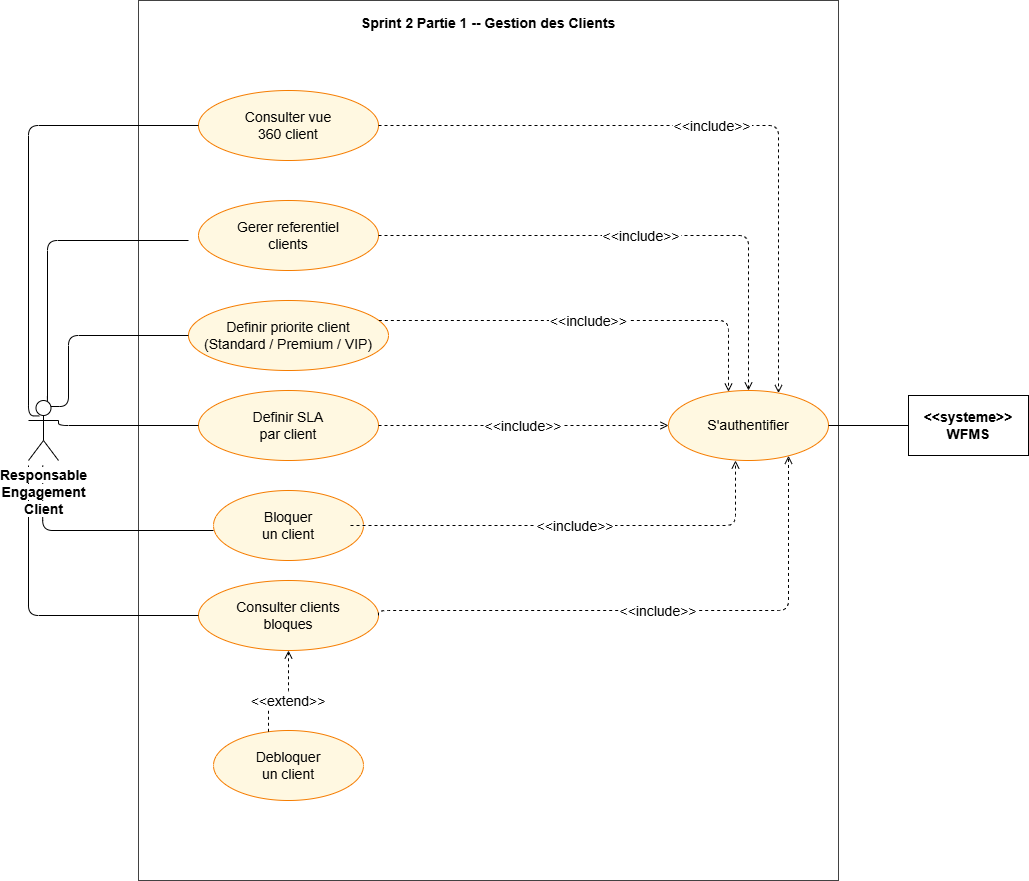
\includegraphics[width=0.9\textwidth, height=0.85\textheight, keepaspectratio]{img/diagrammes/sprint_2_usecase_p1}%
}{%
  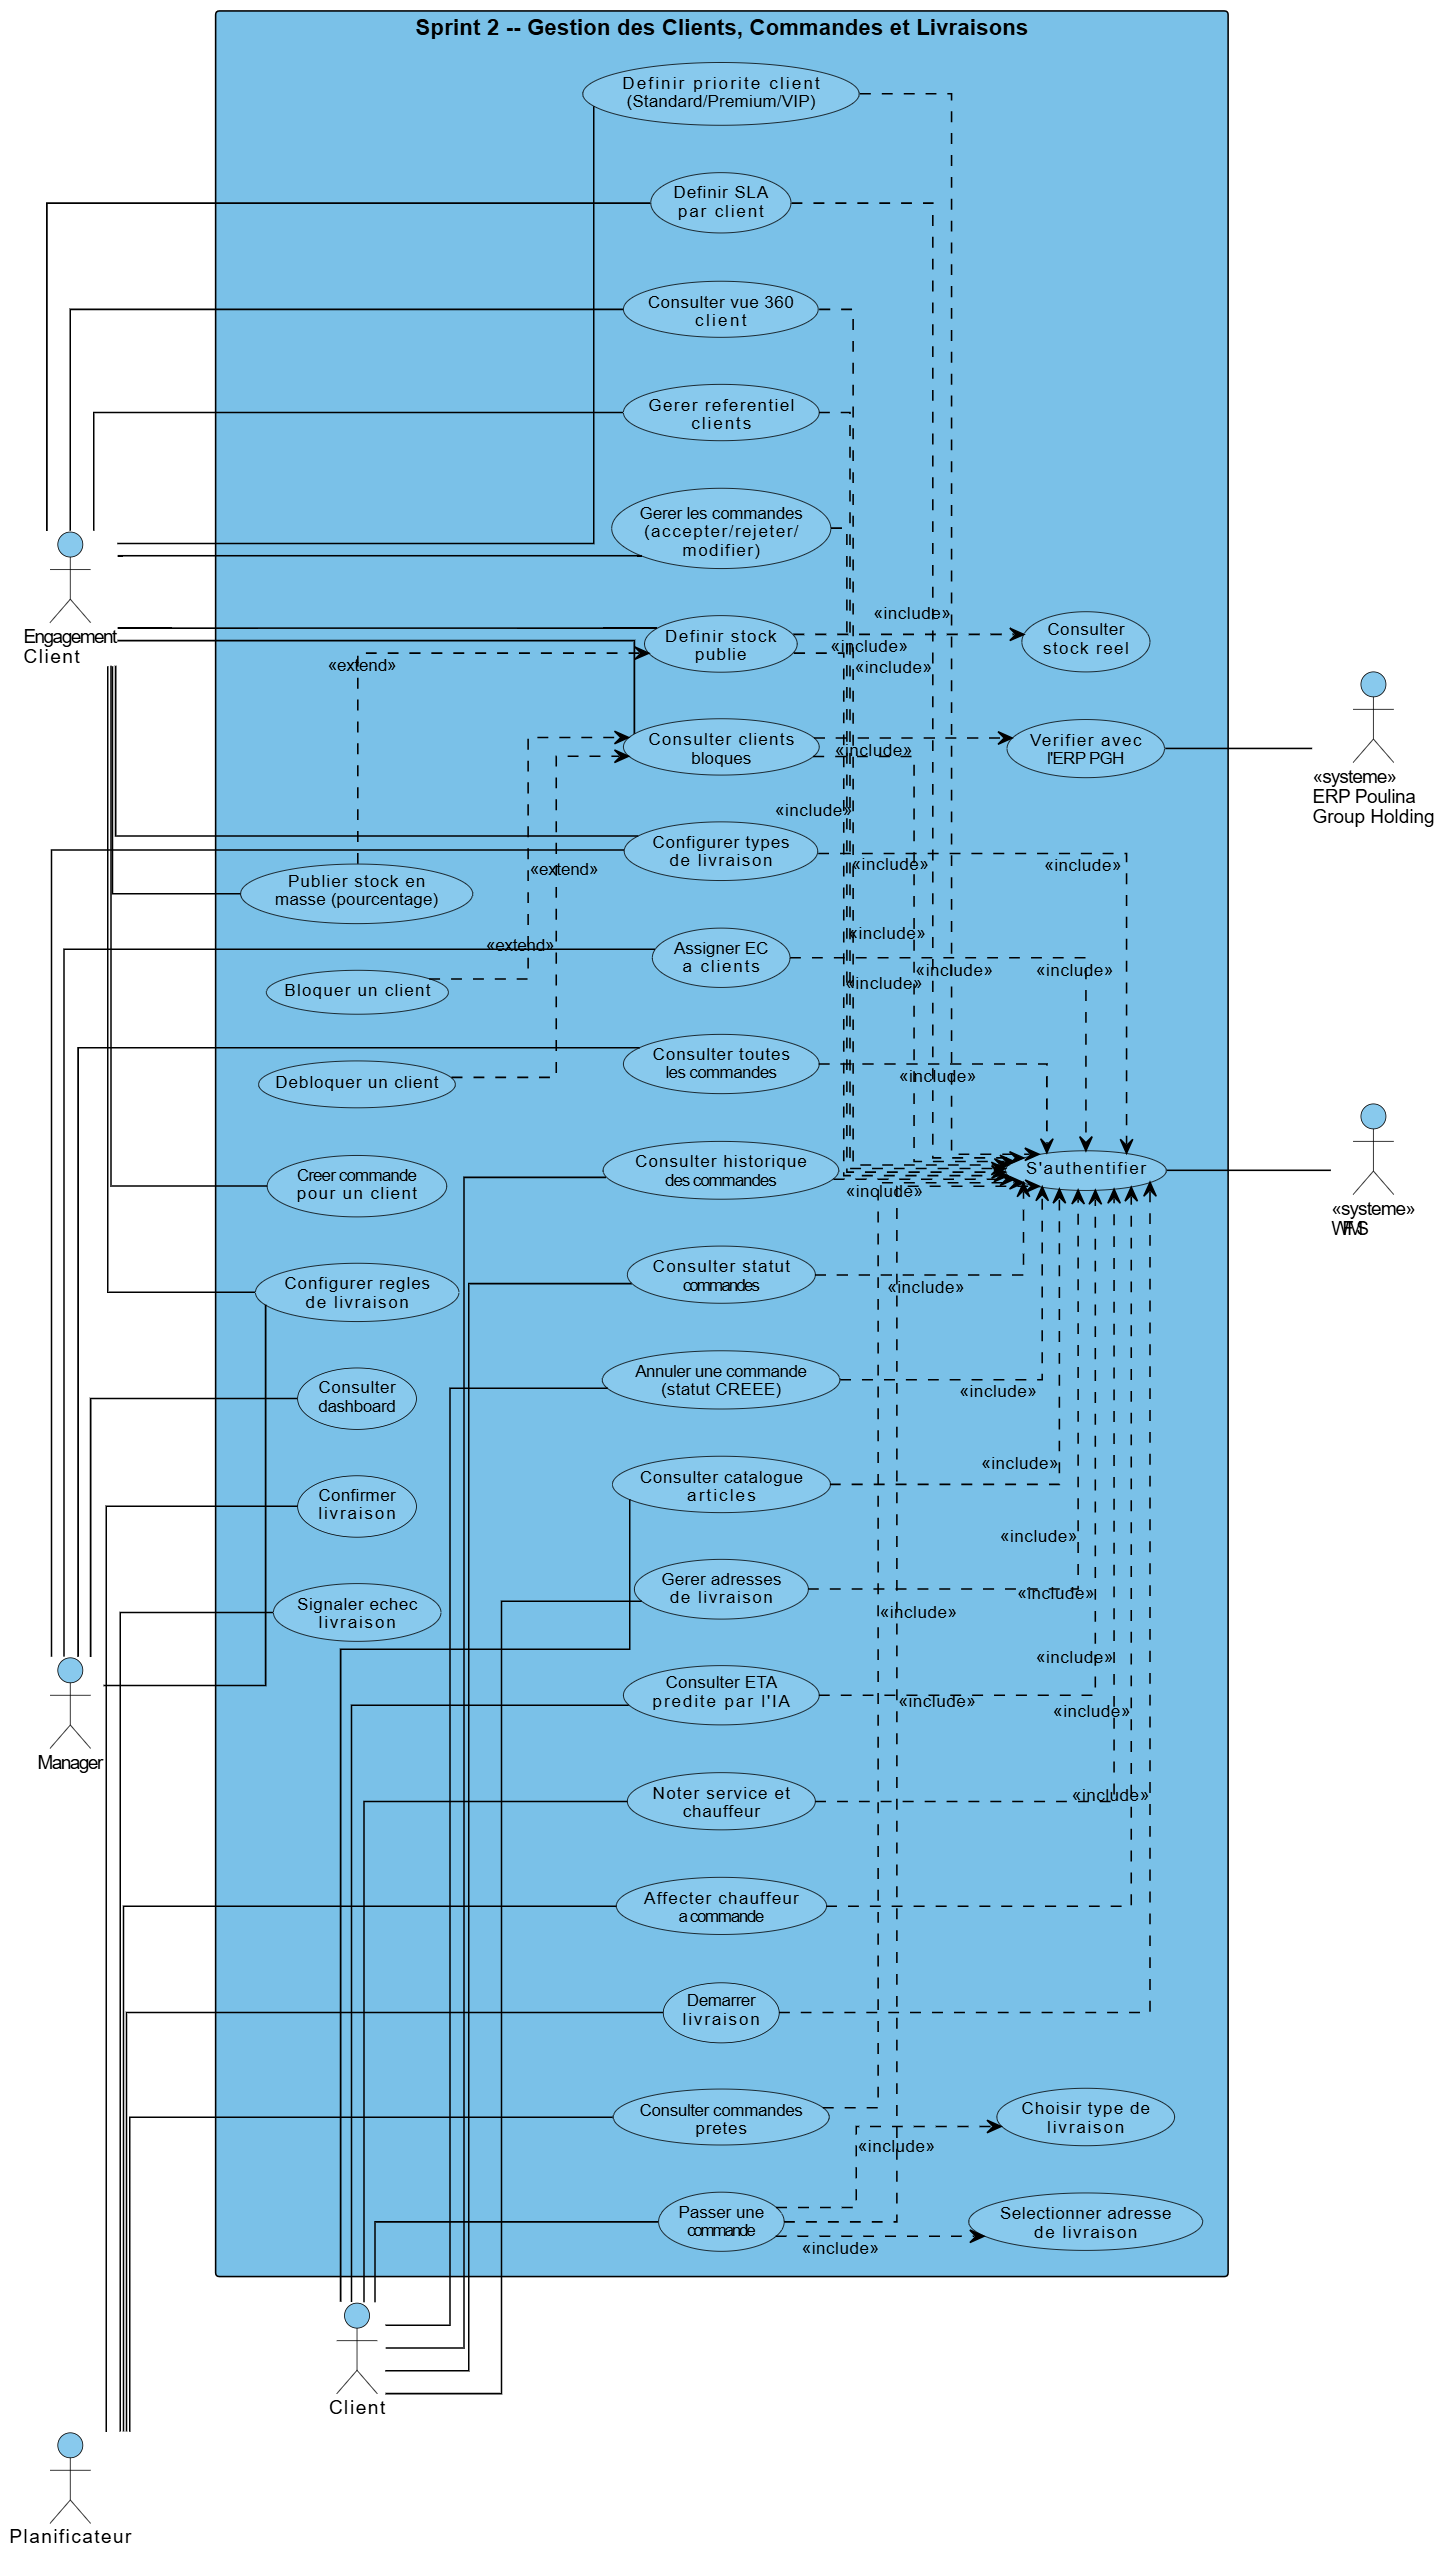
\includegraphics[width=0.9\textwidth, height=0.85\textheight, keepaspectratio]{img/diagrammes/sprint_2_usecase}%
}
\caption{Diagramme de cas d'utilisation du Sprint~2 --- Partie~1}
\label{fig:cas-utilisation-sp2-p1}
\end{figure}

\begin{figure}[H]
\centering
\IfFileExists{img/diagrammes/sprint_2_usecase_p2.png}{%
  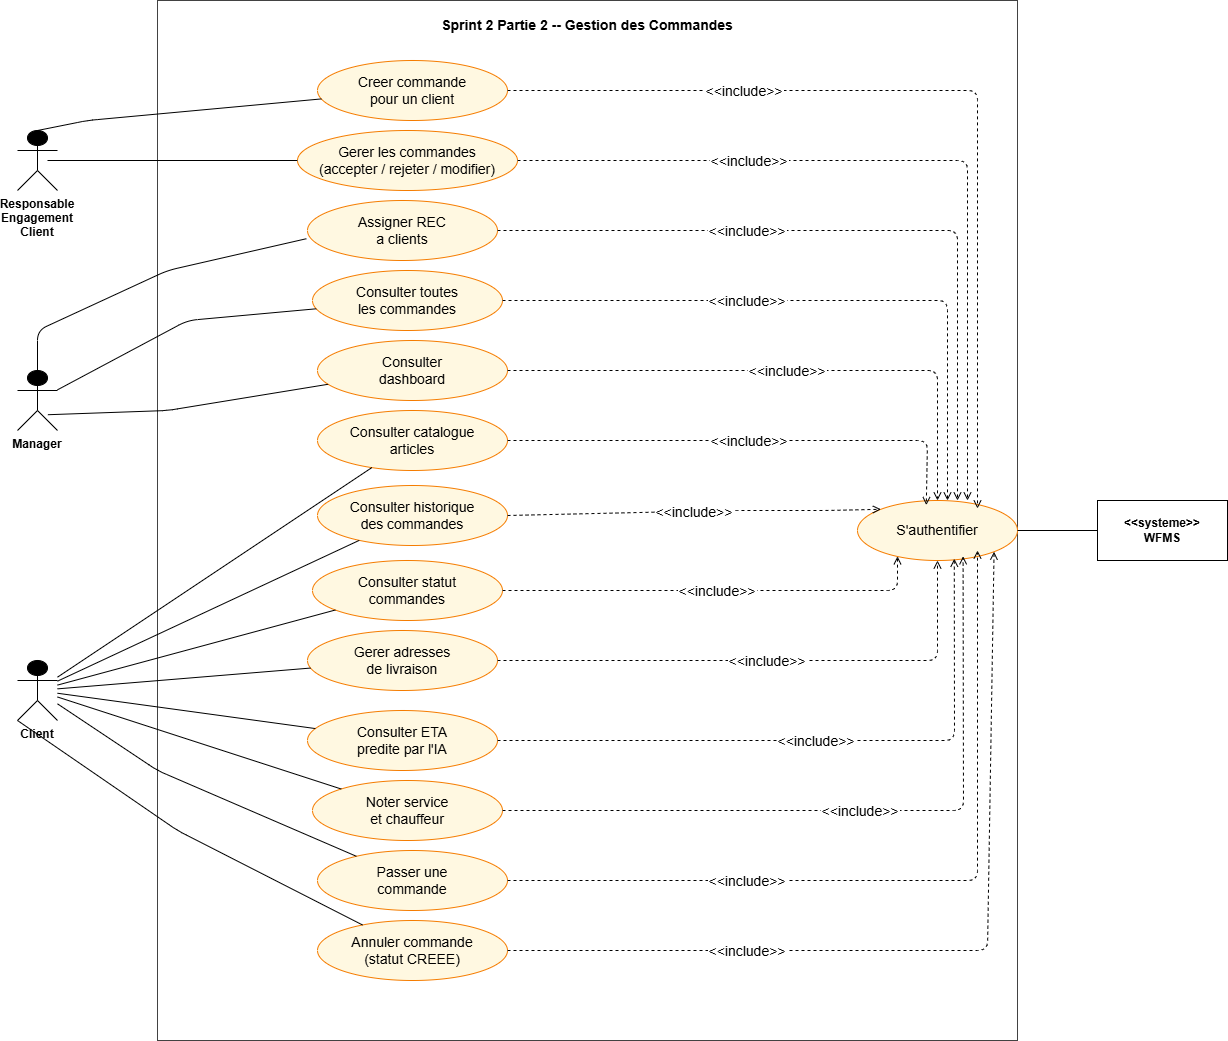
\includegraphics[width=0.9\textwidth, height=0.85\textheight, keepaspectratio]{img/diagrammes/sprint_2_usecase_p2}%
}{%
  \fbox{\parbox{0.9\linewidth}{\centering\vspace{1.5cm}\textit{[img/diagrammes/sprint\_2\_usecase\_p2.png]}\vspace{1.5cm}}}%
}
\caption{Diagramme de cas d'utilisation du Sprint~2 --- Partie~2}
\label{fig:cas-utilisation-sp2-p2}
\end{figure}

\begin{figure}[H]
\centering
\IfFileExists{img/diagrammes/sprint_2_usecase_p3.png}{%
  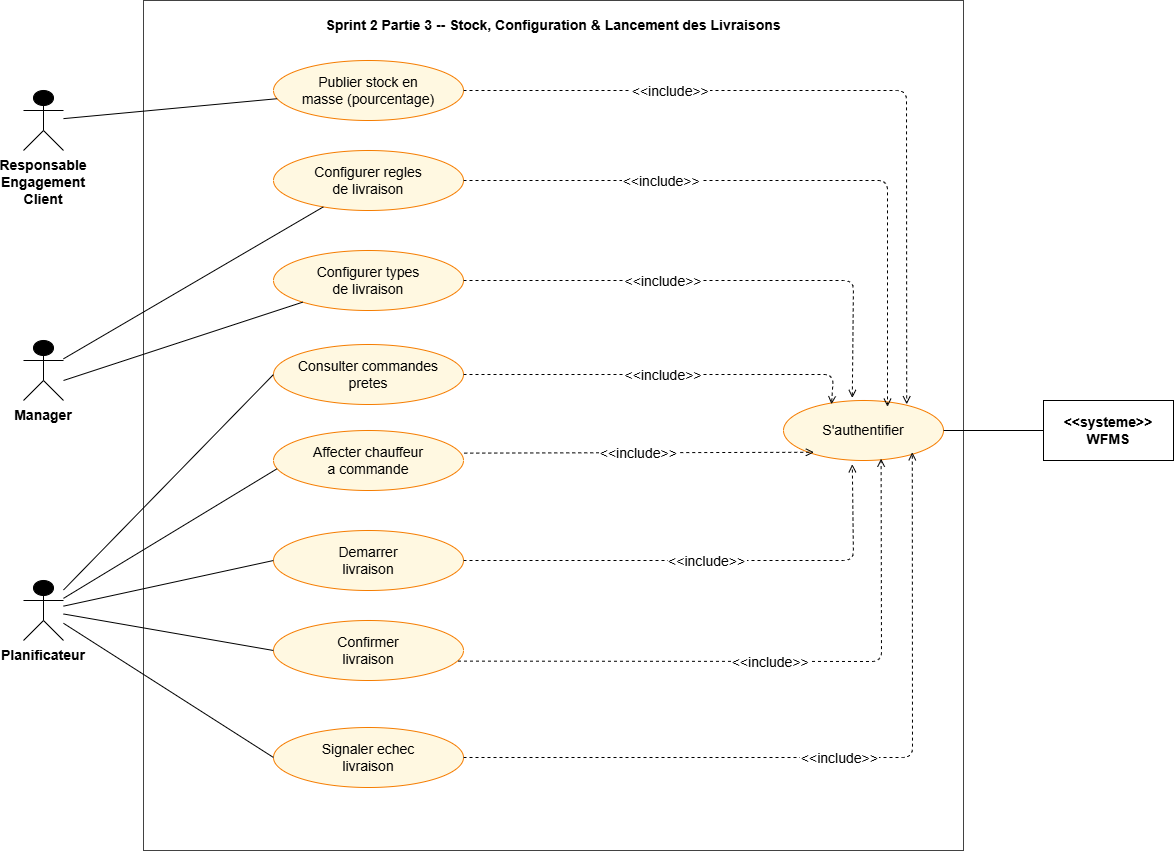
\includegraphics[width=0.9\textwidth, height=0.85\textheight, keepaspectratio]{img/diagrammes/sprint_2_usecase_p3}%
}{%
  \fbox{\parbox{0.9\linewidth}{\centering\vspace{1.5cm}\textit{[img/diagrammes/sprint\_2\_usecase\_p3.png]}\vspace{1.5cm}}}%
}
\caption{Diagramme de cas d'utilisation du Sprint~2 --- Partie~3}
\label{fig:cas-utilisation-sp2-p3}
\end{figure}

\subsection{Description textuelle}

\captionsetup[longtable]{justification=centering}
\setlength{\arrayrulewidth}{1pt}
\begin{longtable}{|p{4cm}|p{11cm}|}
\hline
\rowcolor{headerbg}
\textbf{Élément} & \textbf{Description} \\
\hline
\textbf{Titre} & Gérer les commandes \\
\hline
\textbf{Acteurs} & REC (parties 1, 2, 3), Manager (parties 2, 3), Client (partie 2), Planificateur (partie 3), Système WFMS \\
\hline
\textbf{Objectif} &
\begin{itemize}[nosep, leftmargin=1.4em]
    \item \textbf{P1 :} Maintenir le référentiel clients (vue~360, priorité Standard/Premium/VIP, SLA, blocage/déblocage).
    \item \textbf{P2 :} Gérer le cycle de vie des commandes (création, acceptation/rejet, suivi ETA par IA) pour le REC, le Manager et le Client.
    \item \textbf{P3 :} Configurer le stock et les règles de livraison, affecter les chauffeurs et lancer les missions.
\end{itemize} \\
\hline
\textbf{Précondition} & Tous les acteurs sont authentifiés via WFMS. Le catalogue produits, le stock et les règles de livraison sont disponibles. \\
\hline
\textbf{Postcondition} & Le référentiel clients est à jour~; la commande est transmise à l'ERP (statut ACCEPTÉE)~; les livraisons sont affectées et leur statut (confirmée ou échec) est enregistré. \\
\hline
\textbf{Scénario nominal} &
\begin{enumerate}[start=1, label=\arabic*., nosep, leftmargin=1.4em]
    \item Le REC met à jour la priorité et le SLA du client depuis la vue~360.
    \item Le Client passe une commande~; le REC la crée, vérifie le stock et l'accepte (statut ACCEPTÉE) — la commande est envoyée à l'ERP.
    \item Le Manager pilote via le dashboard~; le Client suit l'état et consulte l'ETA prédit par IA.
    \item Le REC publie le stock en masse et configure les règles/types de livraison.
    \item Le Planificateur consulte les commandes prêtes, affecte un chauffeur, démarre et confirme la livraison.
\end{enumerate} \\
\hline
\textbf{Scénario alternatif} &
\begin{enumerate}[start=1, label=\arabic*., nosep, leftmargin=1.4em]
    \item Client bloqué : commande refusée~; le REC peut débloquer après régularisation.
    \item Stock insuffisant : création bloquée~; le REC publie une mise à jour de stock en masse.
    \item Commande rejetée par le REC : le Client est notifié et peut l'annuler (statut CRÉÉE uniquement).
    \item Échec de livraison : le Planificateur le signale~; la mission est replanifiée.
\end{enumerate} \\
\hline
\caption{Description textuelle --- Gérer les commandes (Sprint 2)}
\end{longtable}
\setlength{\arrayrulewidth}{0.4pt}

\subsection{Cycle de vie d'une commande}

La figure~\ref{fig:cycle-vie-commande-sp2} illustre le cycle de vie complet d'une commande Fleet AI depuis sa création jusqu'à la livraison, en montrant les interactions entre le Client, le REC, l'ERP Poulina et le système de livraison.

\begin{figure}[H]
\centering
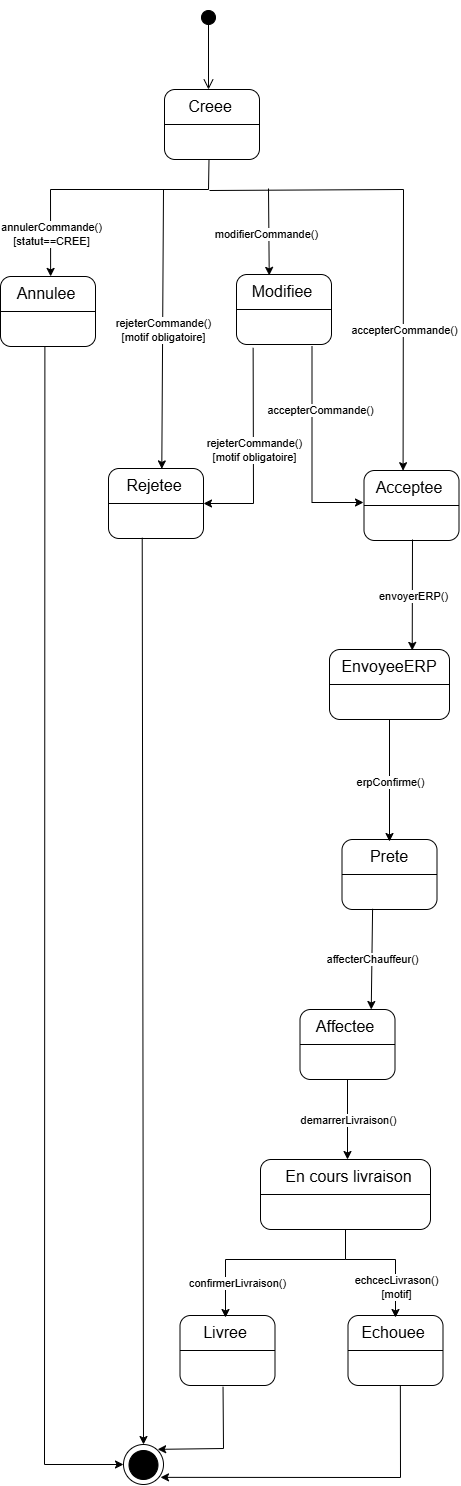
\includegraphics[width=\textwidth, height=0.7\textheight, keepaspectratio]{img/diagrammes/sprint2_cycleVieCommande}
\caption{Cycle de vie complet d'une commande Fleet AI}
\label{fig:cycle-vie-commande-sp2}
\end{figure}

\subsection{Diagramme de classes}

\newpage
\thispagestyle{empty}
\begin{landscape}
\begin{figure}[H]
\centering
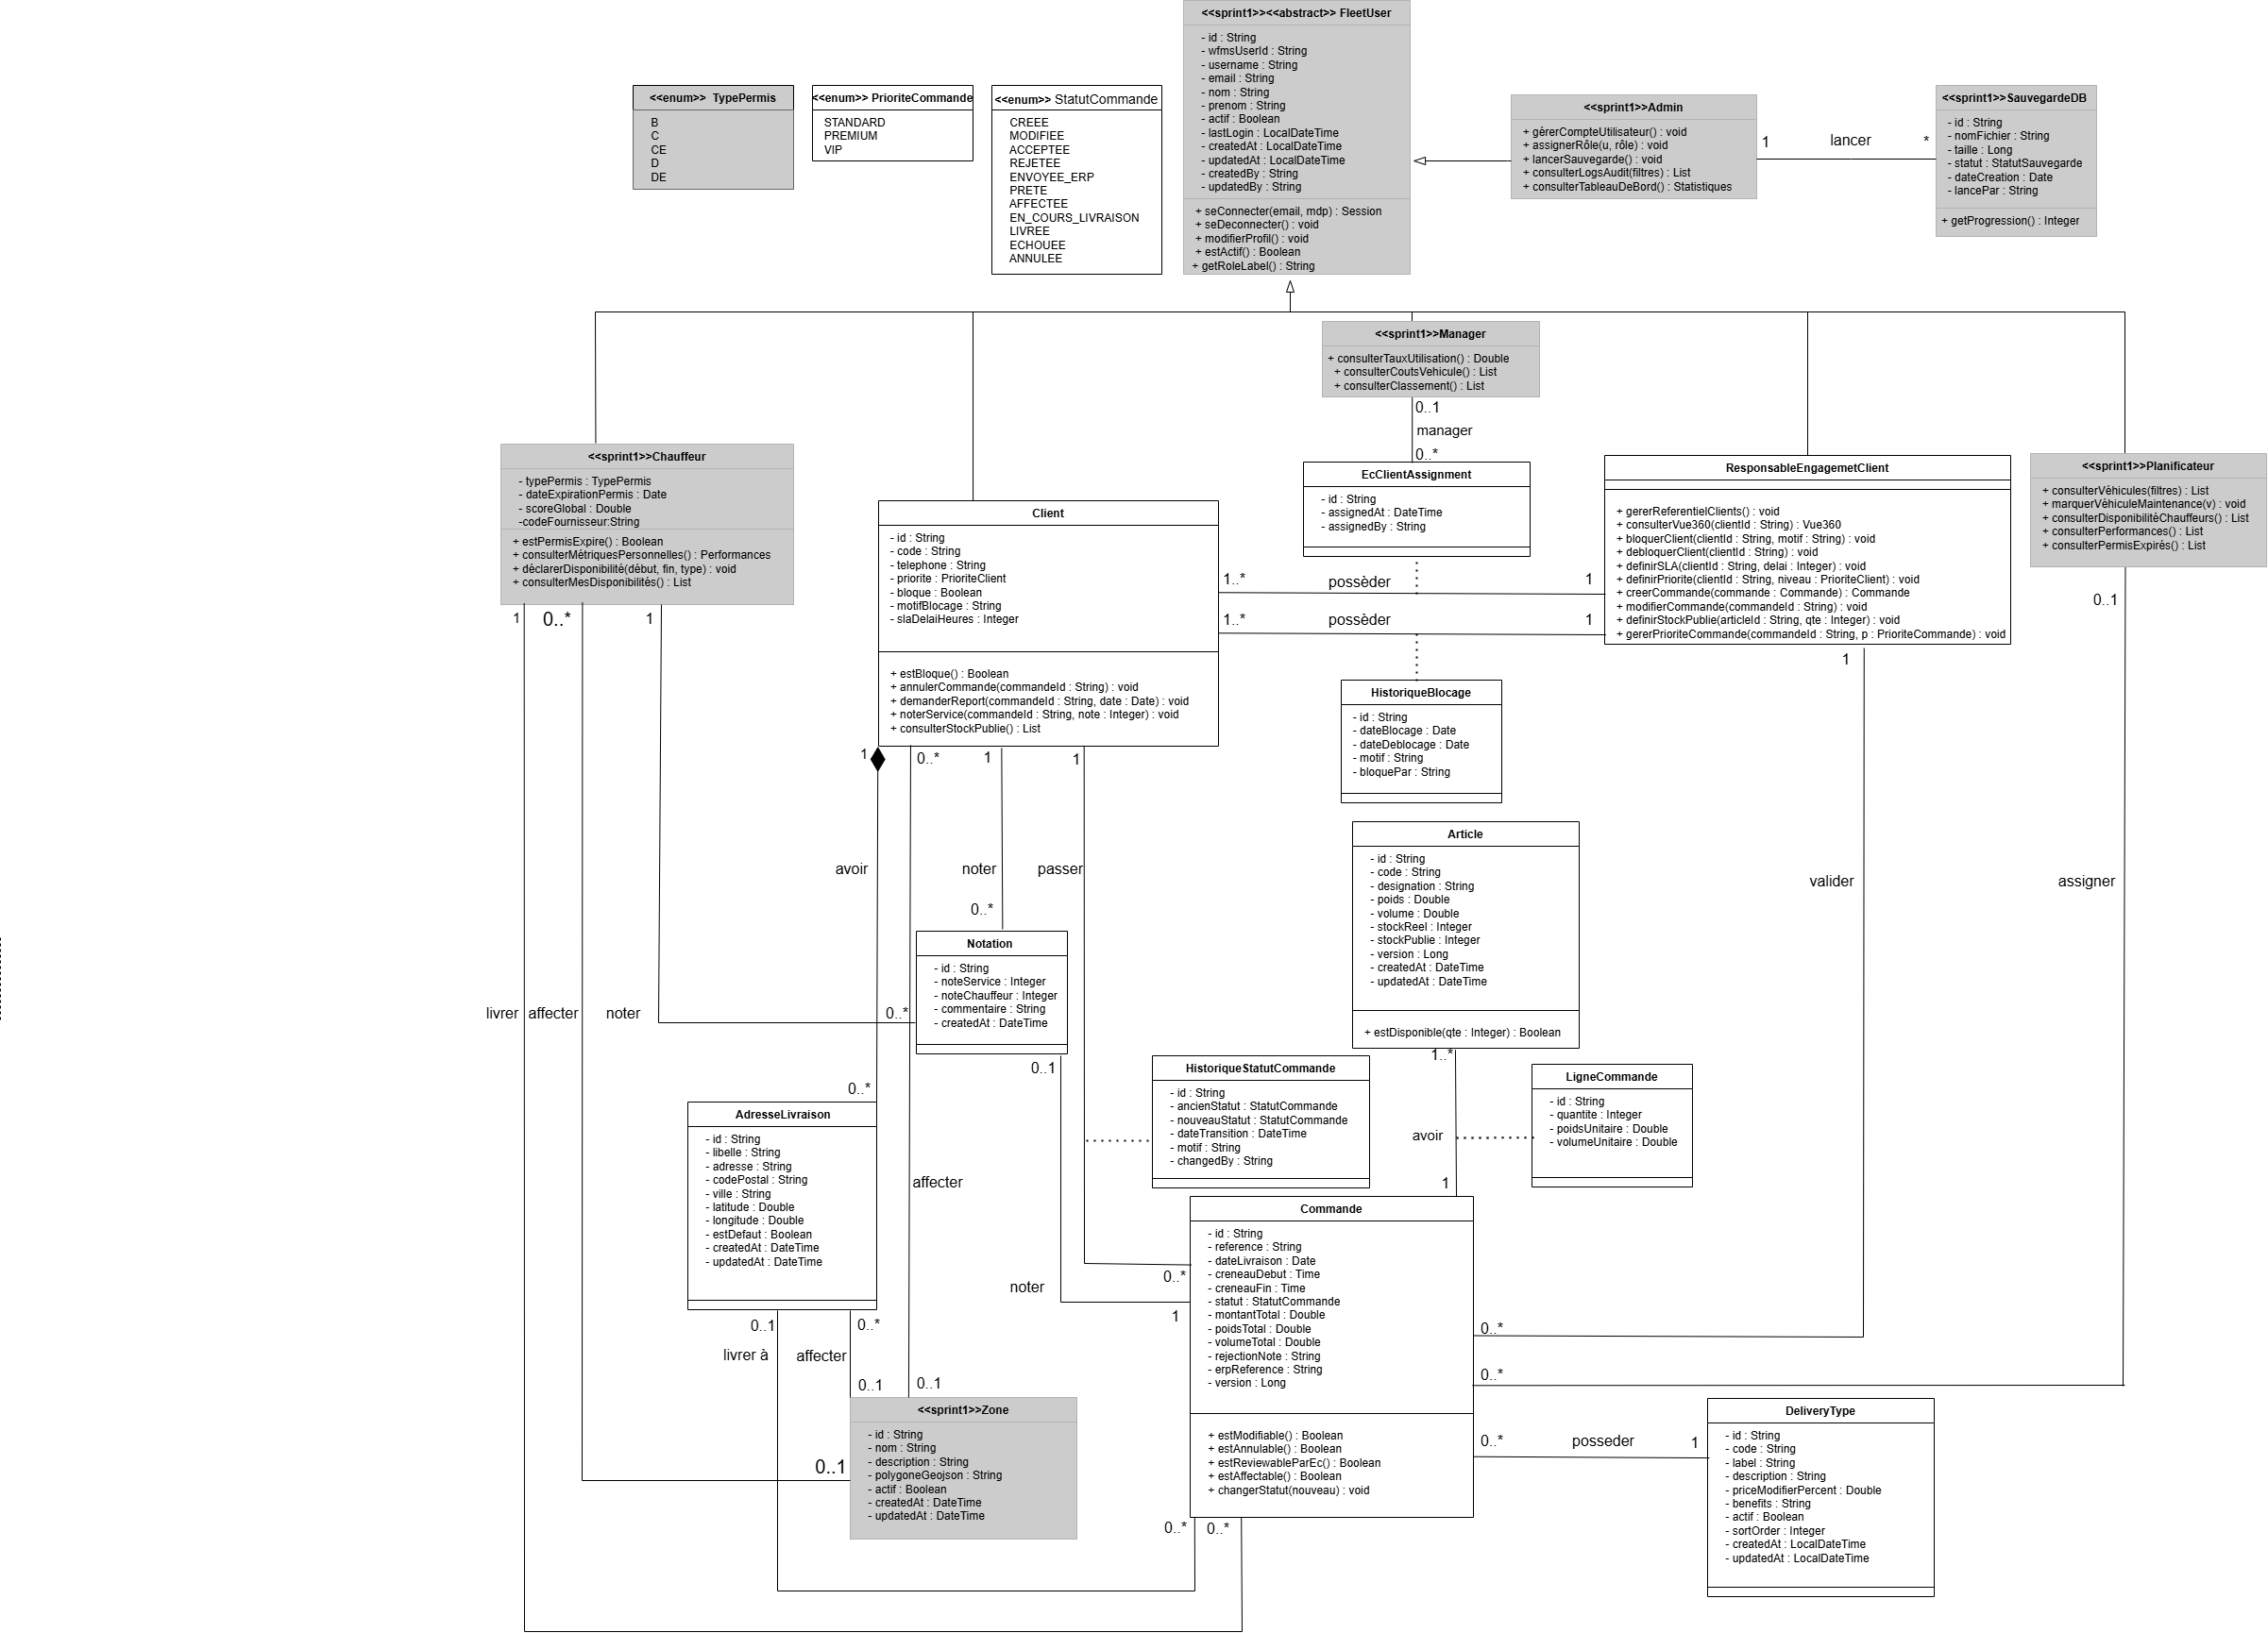
\includegraphics[width=\linewidth, height=0.95\textheight, keepaspectratio]{img/diagrammes/sprint_2_classes}
\caption{Diagramme de classes du Sprint 2}
\label{fig:diag-classes-sp2}
\end{figure}
\end{landscape}

% =============================================================
\section{Réalisation}
% =============================================================

\subsection{Gestion des clients et adresses de livraison}

Le REC gère son portefeuille via une liste paginable avec filtres. La Vue 360° d'un client regroupe ses commandes, ses adresses et son historique de blocage. Le blocage est immédiat avec motif obligatoire. Le REC gère également les adresses de livraison de ses clients, avec détection automatique de la zone de livraison à partir des coordonnées GPS (algorithme Ray-Casting). Une seule adresse peut être marquée comme adresse par défaut.

\begin{figure}[H]
\centering
\IfFileExists{img/capture/web/sp2_clients_composite.png}{%
  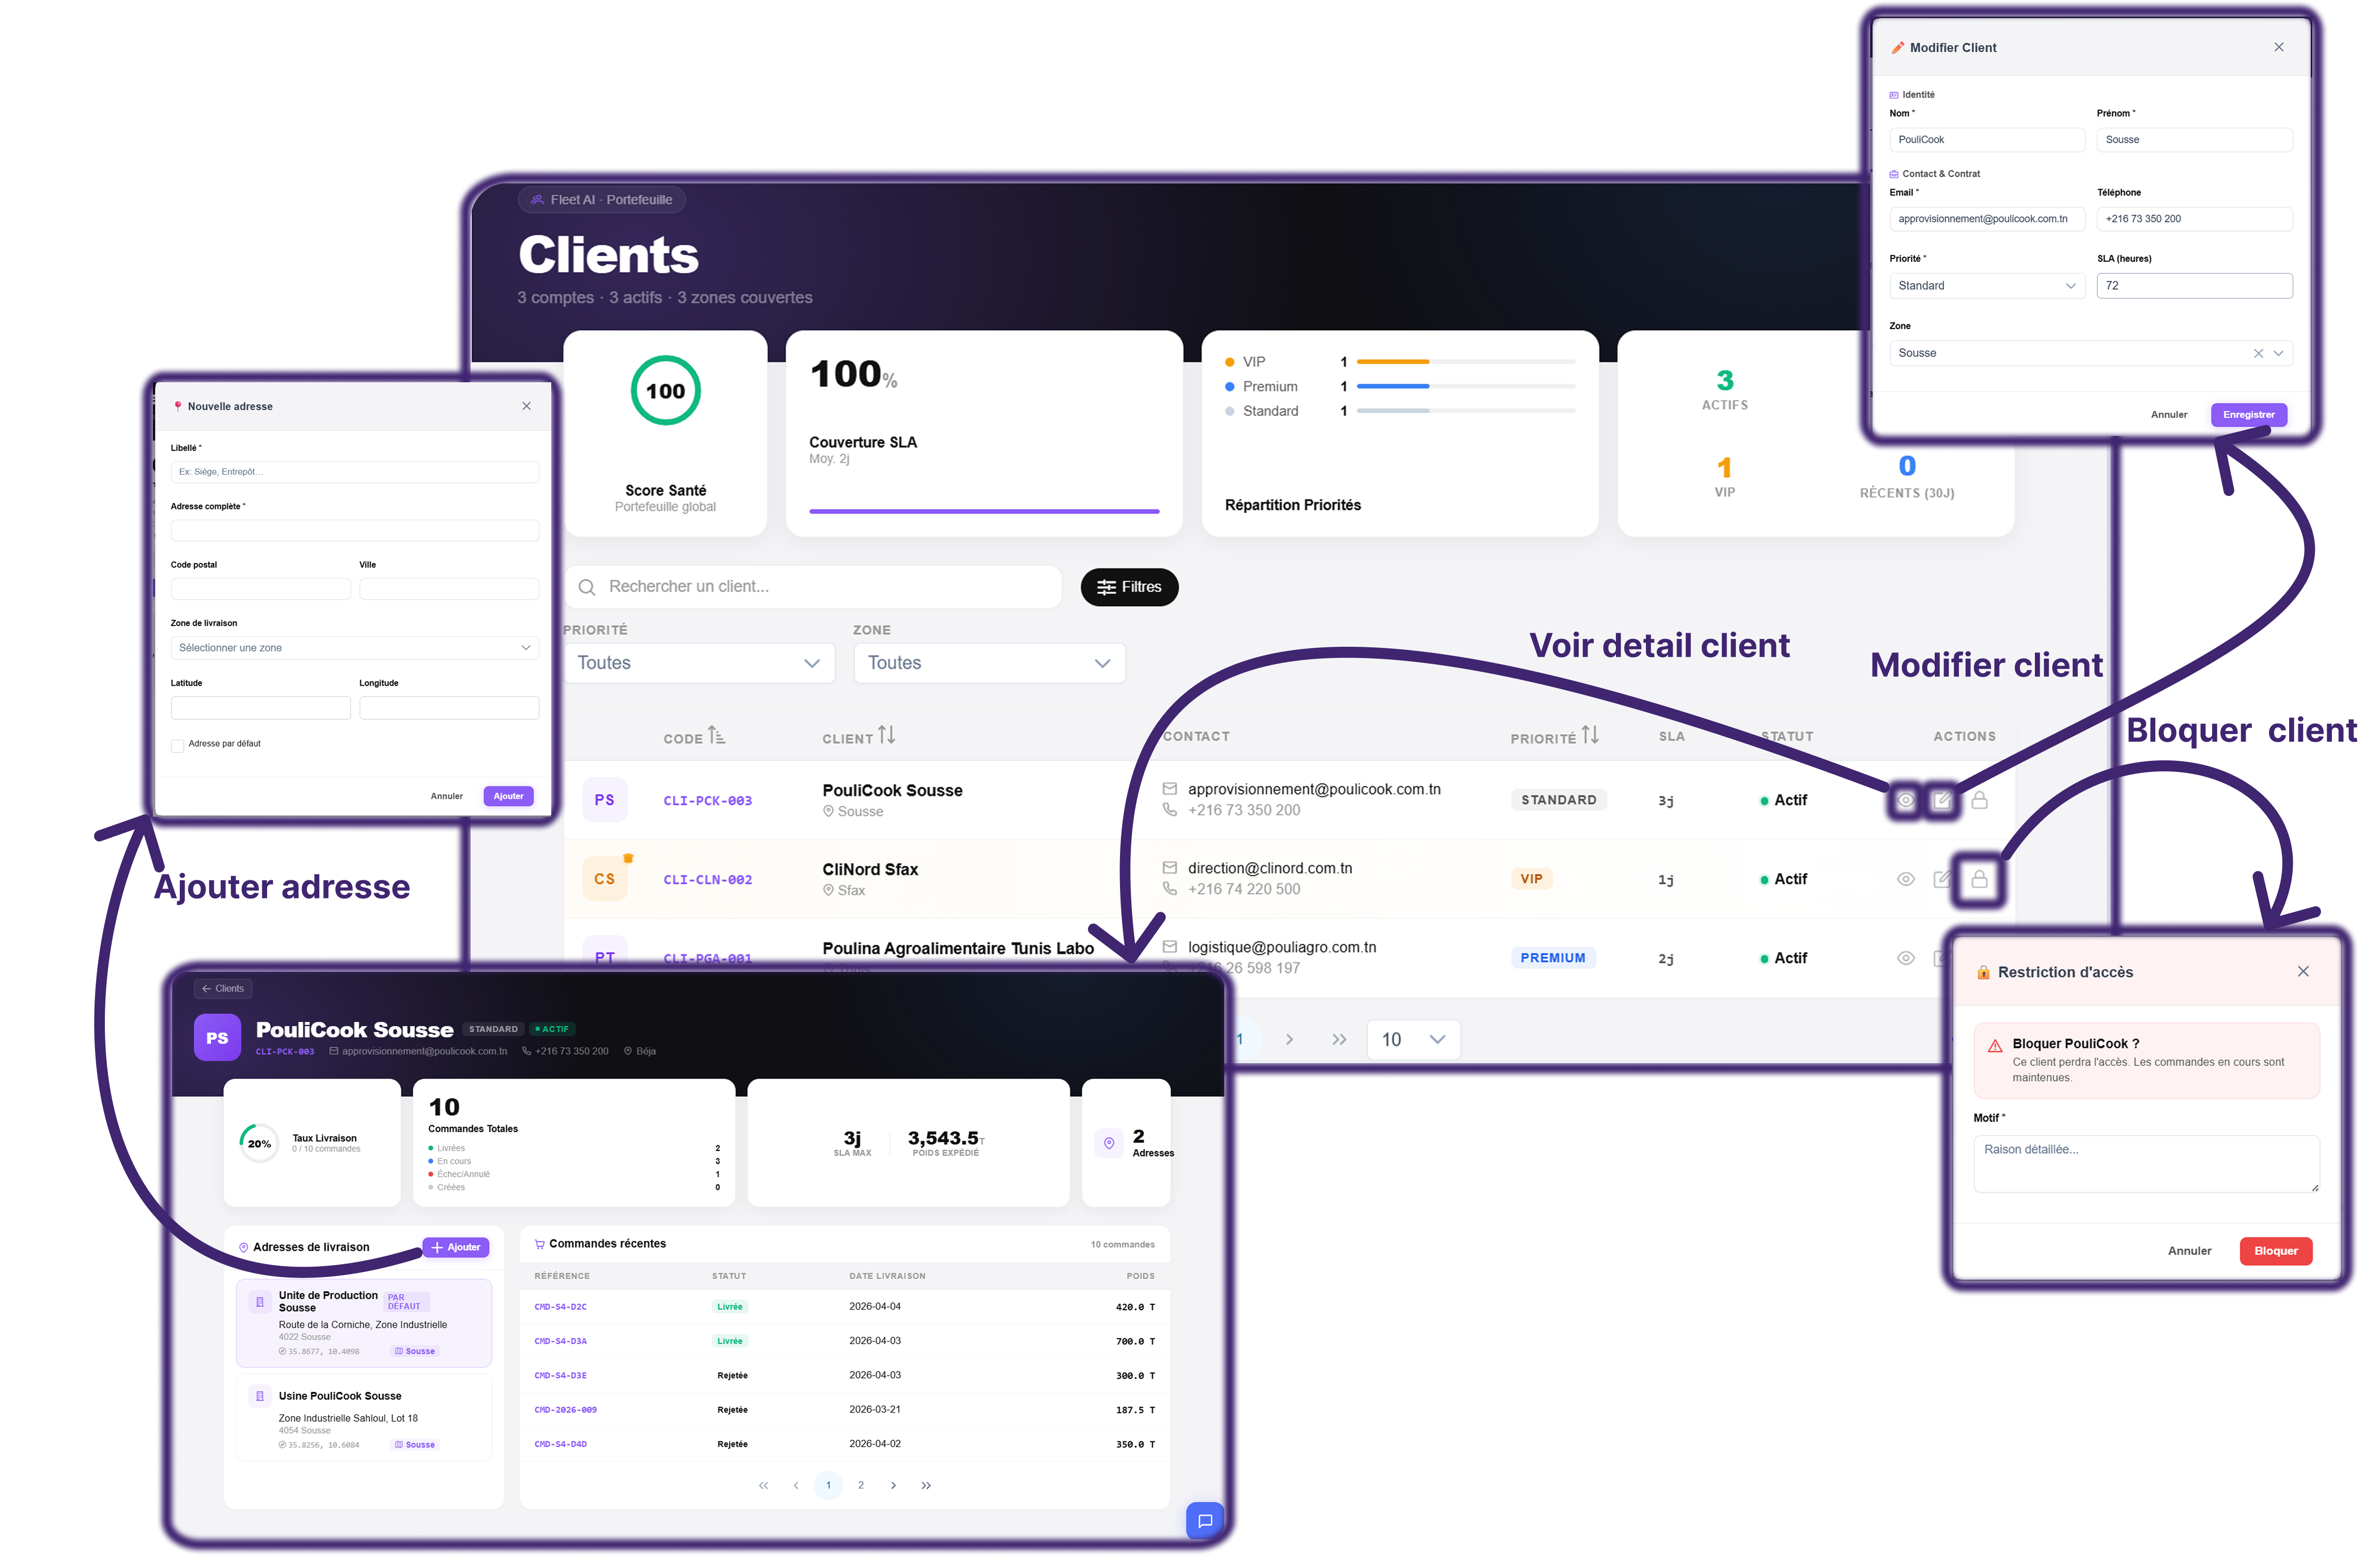
\includegraphics[width=\linewidth, keepaspectratio]{img/capture/web/sp2_clients_composite}%
}{%
  \fbox{\parbox{0.9\linewidth}{\centering\vspace{1.5cm}\textit{[img/sp2\_clients\_composite]}\vspace{1.5cm}}}%
}
\caption{Gestion clients : Vue 360°, blocage et adresses GPS}
\label{fig:sp2-clients-addresses}
\end{figure}

\subsection{Catalogue et gestion du stock}

Deux niveaux de stock coexistent : le stock réel (visible REC uniquement) et le stock publié (visible Client). Le REC fixe manuellement le stock publié dans la limite du stock réel.

\begin{figure}[H]
\centering
\IfFileExists{img/capture/web/sp2_stock_composite.png}{%
  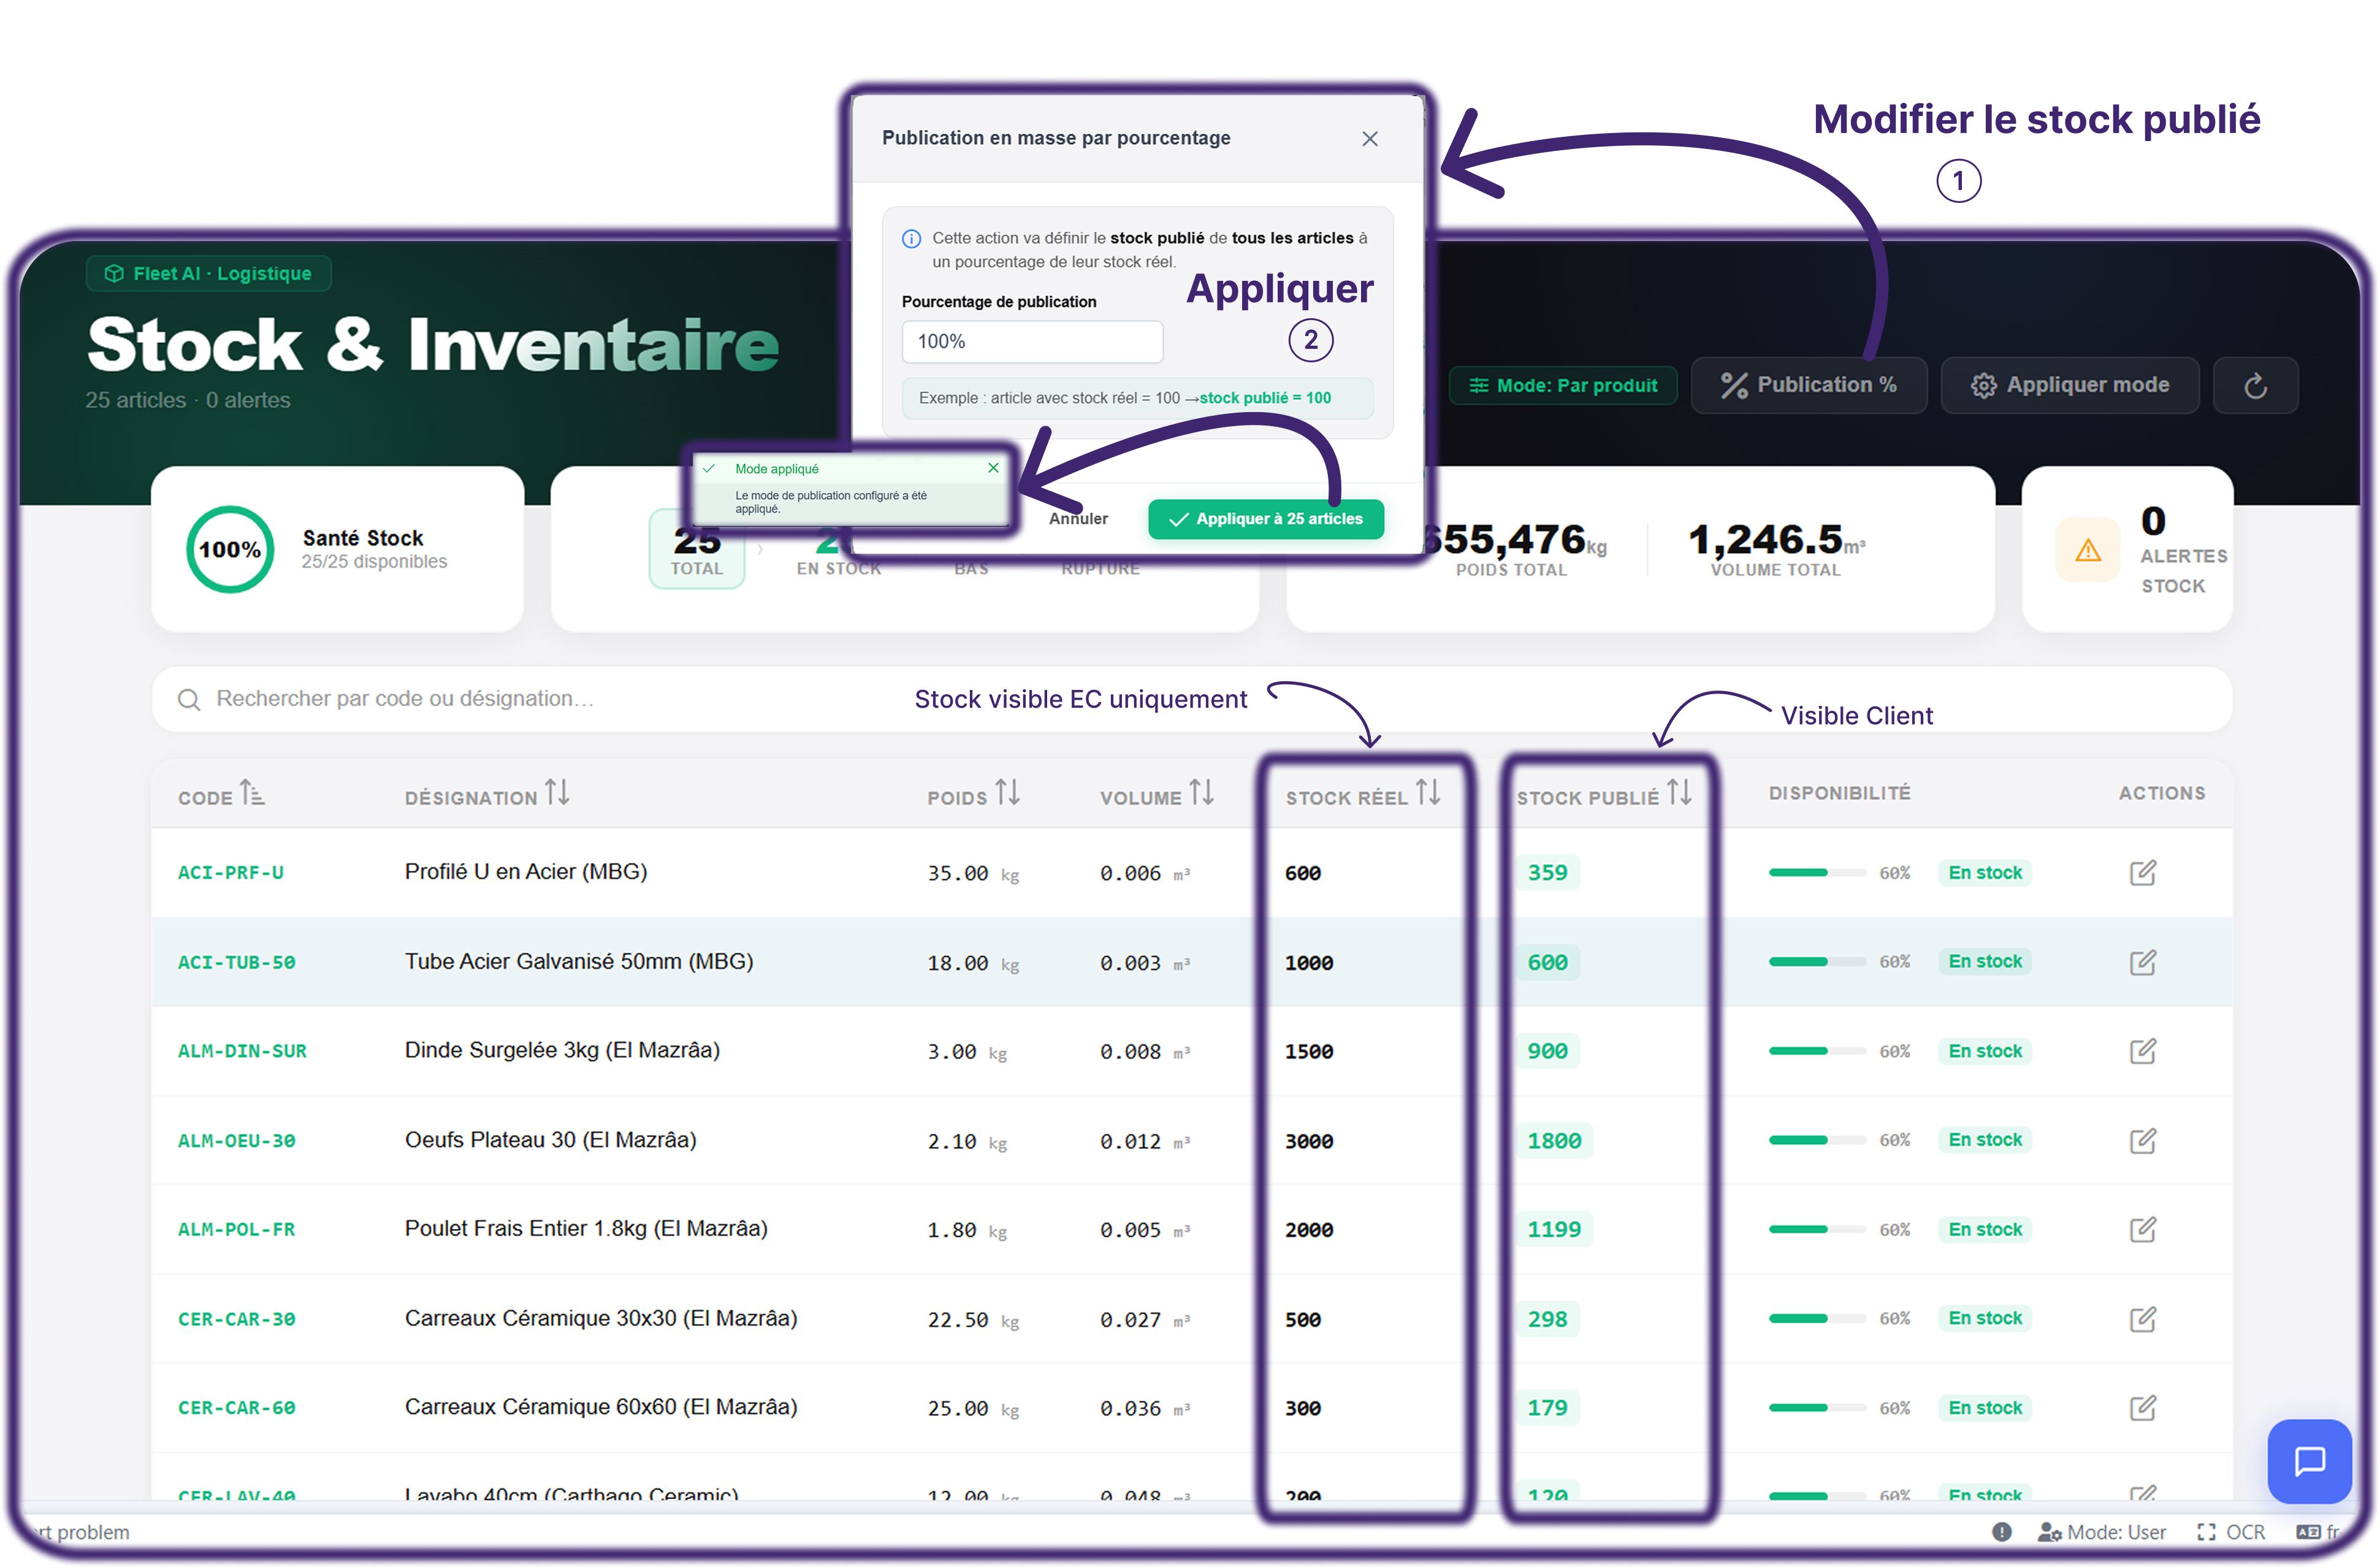
\includegraphics[width=\linewidth, keepaspectratio]{img/capture/web/sp2_stock_composite}%
}{%
  \fbox{\parbox{0.9\linewidth}{\centering\vspace{1.5cm}\textit{[img/sp2\_stock\_composite]}\vspace{1.5cm}}}%
}
\caption{Catalogue : niveaux stock réel et publié}
\label{fig:sp2-stock}
\end{figure}

\subsection{Gestion des commandes}

La création d'une commande vérifie le statut de blocage du client et la disponibilité du stock. La commande suit un cycle de vie strict à dix statuts, chaque transition tracée avec acteur et horodatage.

\begin{figure}[H]
\centering
\IfFileExists{img/capture/web/sp2_orders_composite.png}{%
  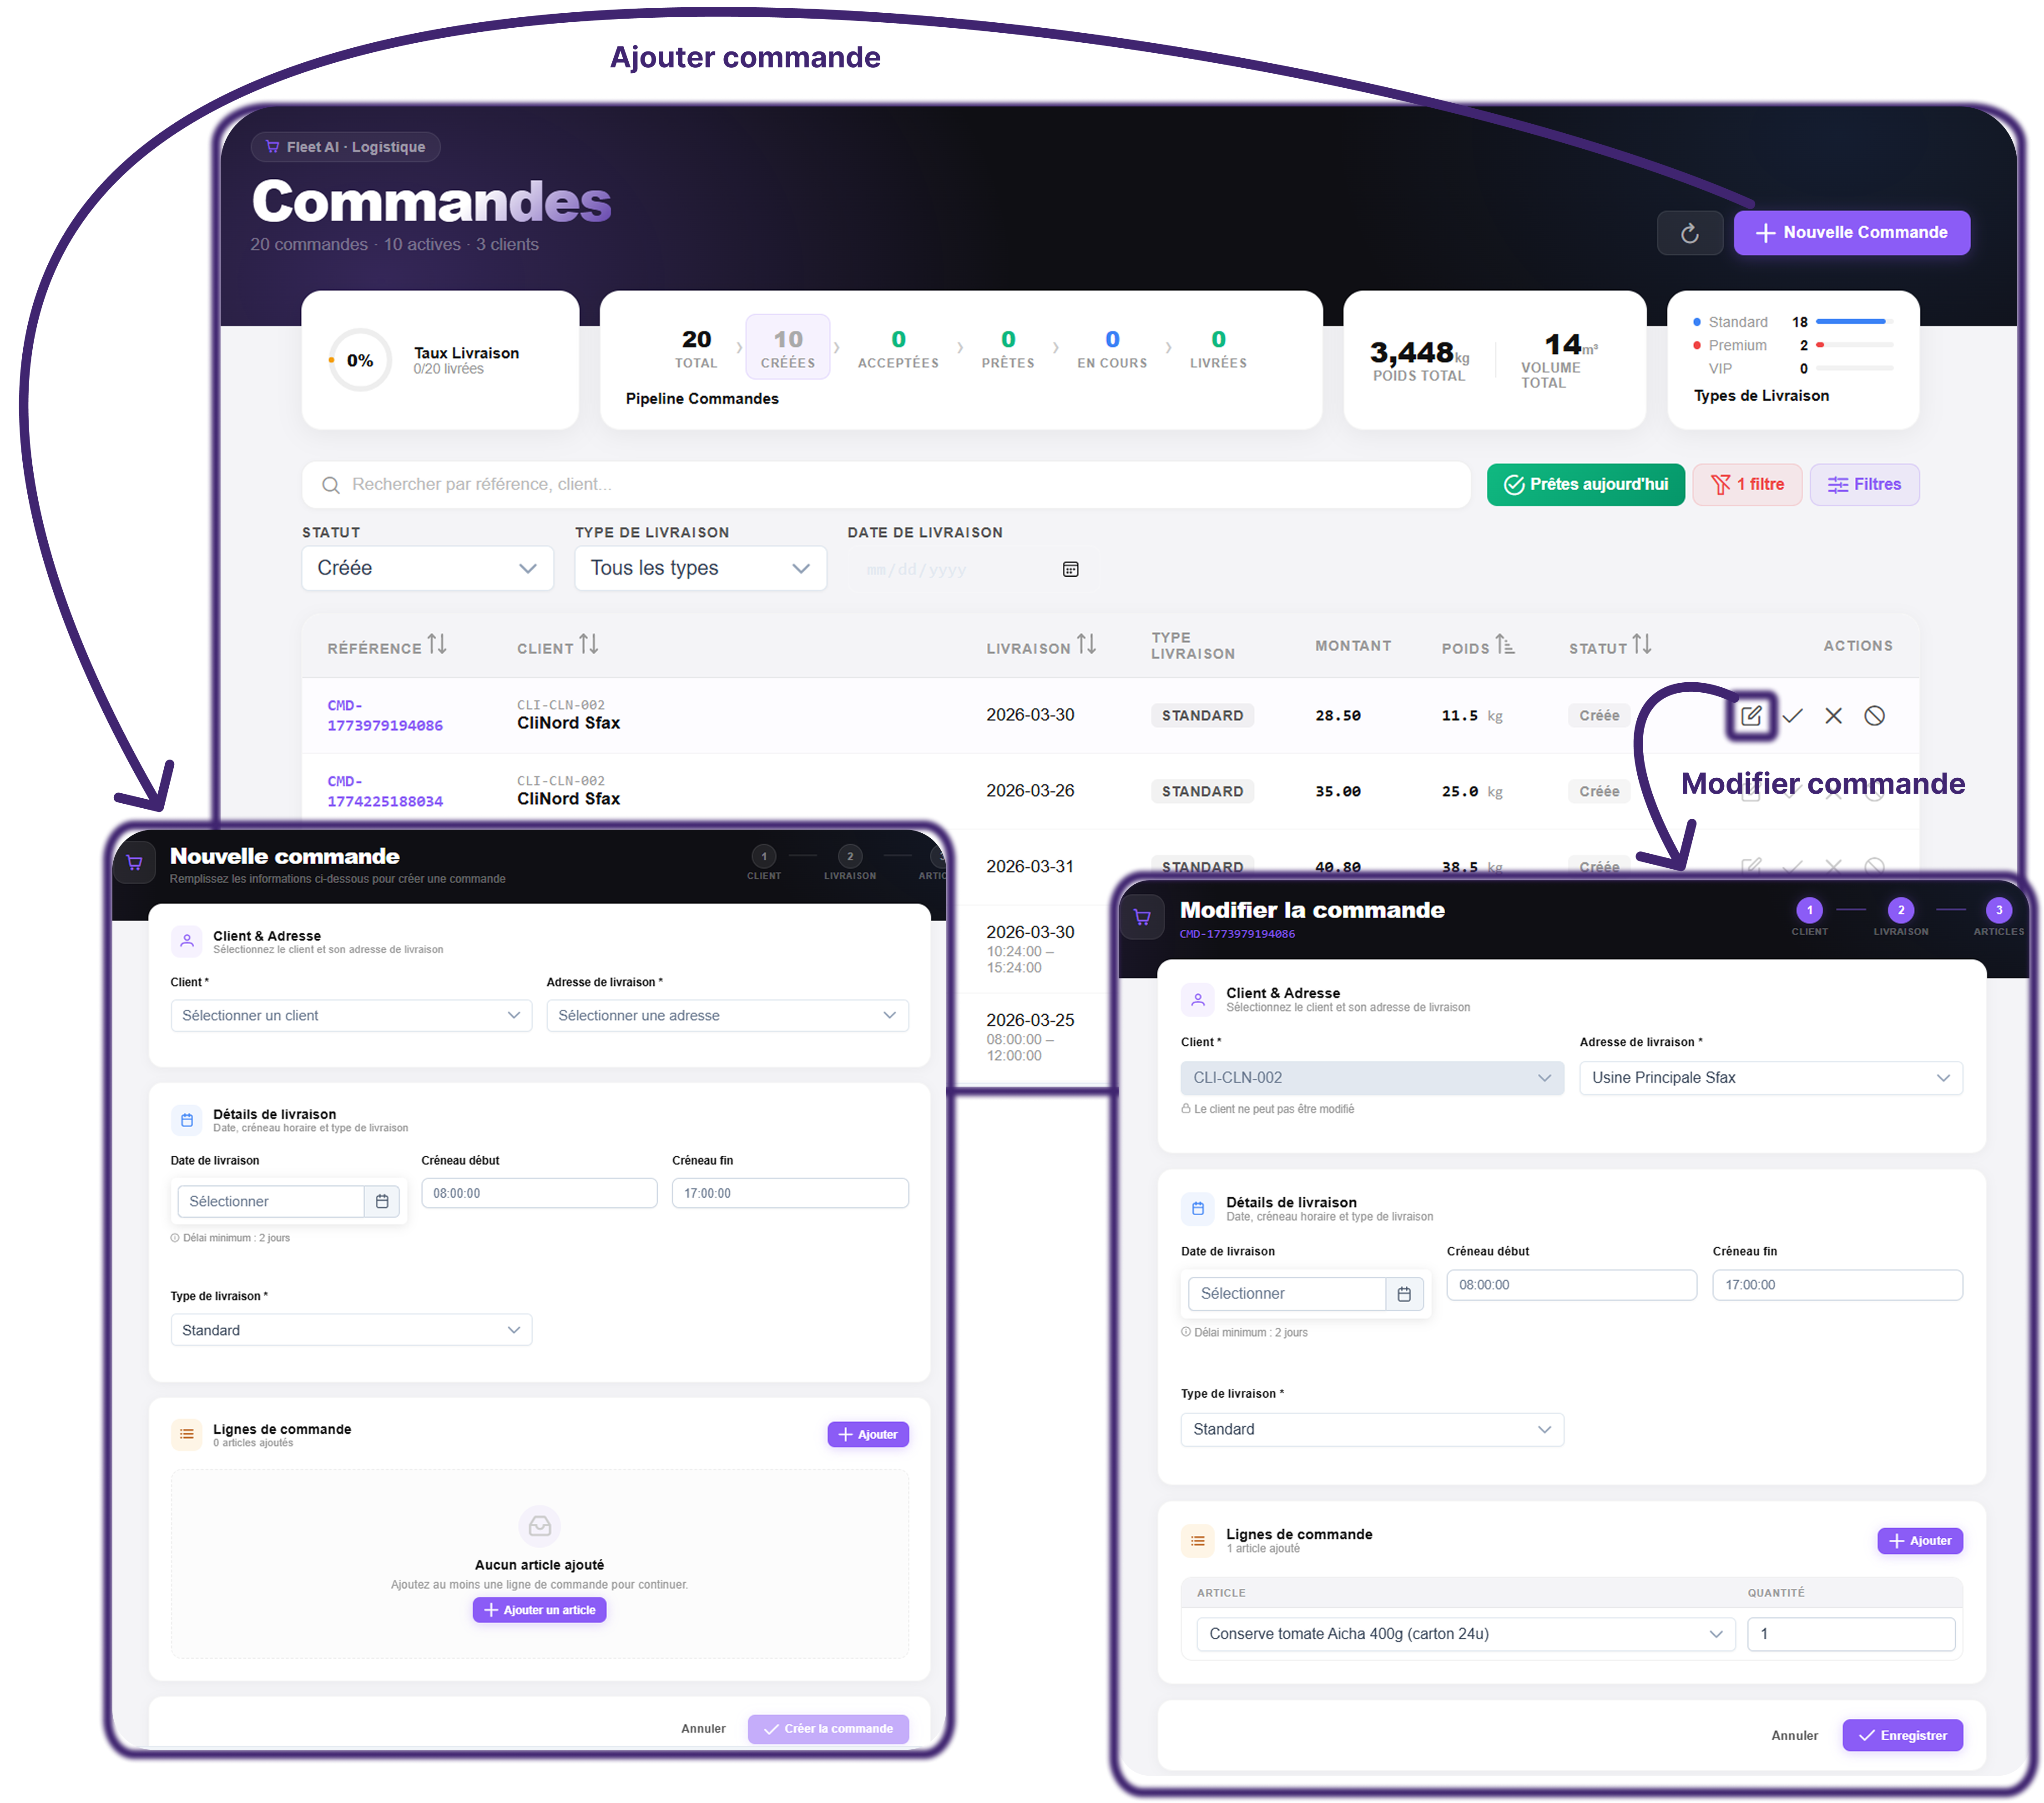
\includegraphics[width=\linewidth, keepaspectratio]{img/capture/web/sp2_orders_composite}%
}{%
  \fbox{\parbox{0.9\linewidth}{\centering\vspace{1.5cm}\textit{[img/sp2\_orders\_composite]}\vspace{1.5cm}}}%
}
\caption{Commandes : badge de statut et formulaire de création}
\label{fig:sp2-orders}
\end{figure}

\subsection{Affectation REC-Client}

Le Manager définit les périmètres de responsabilité en assignant des clients à des REC. Un client ne peut être assigné qu'à un seul REC à la fois. Les affectations et désaffectations en lot sont possibles depuis l'interface dédiée.

\begin{figure}[H]
\centering
\IfFileExists{img/capture/web/sp2_ec_assignments_composite.png}{%
  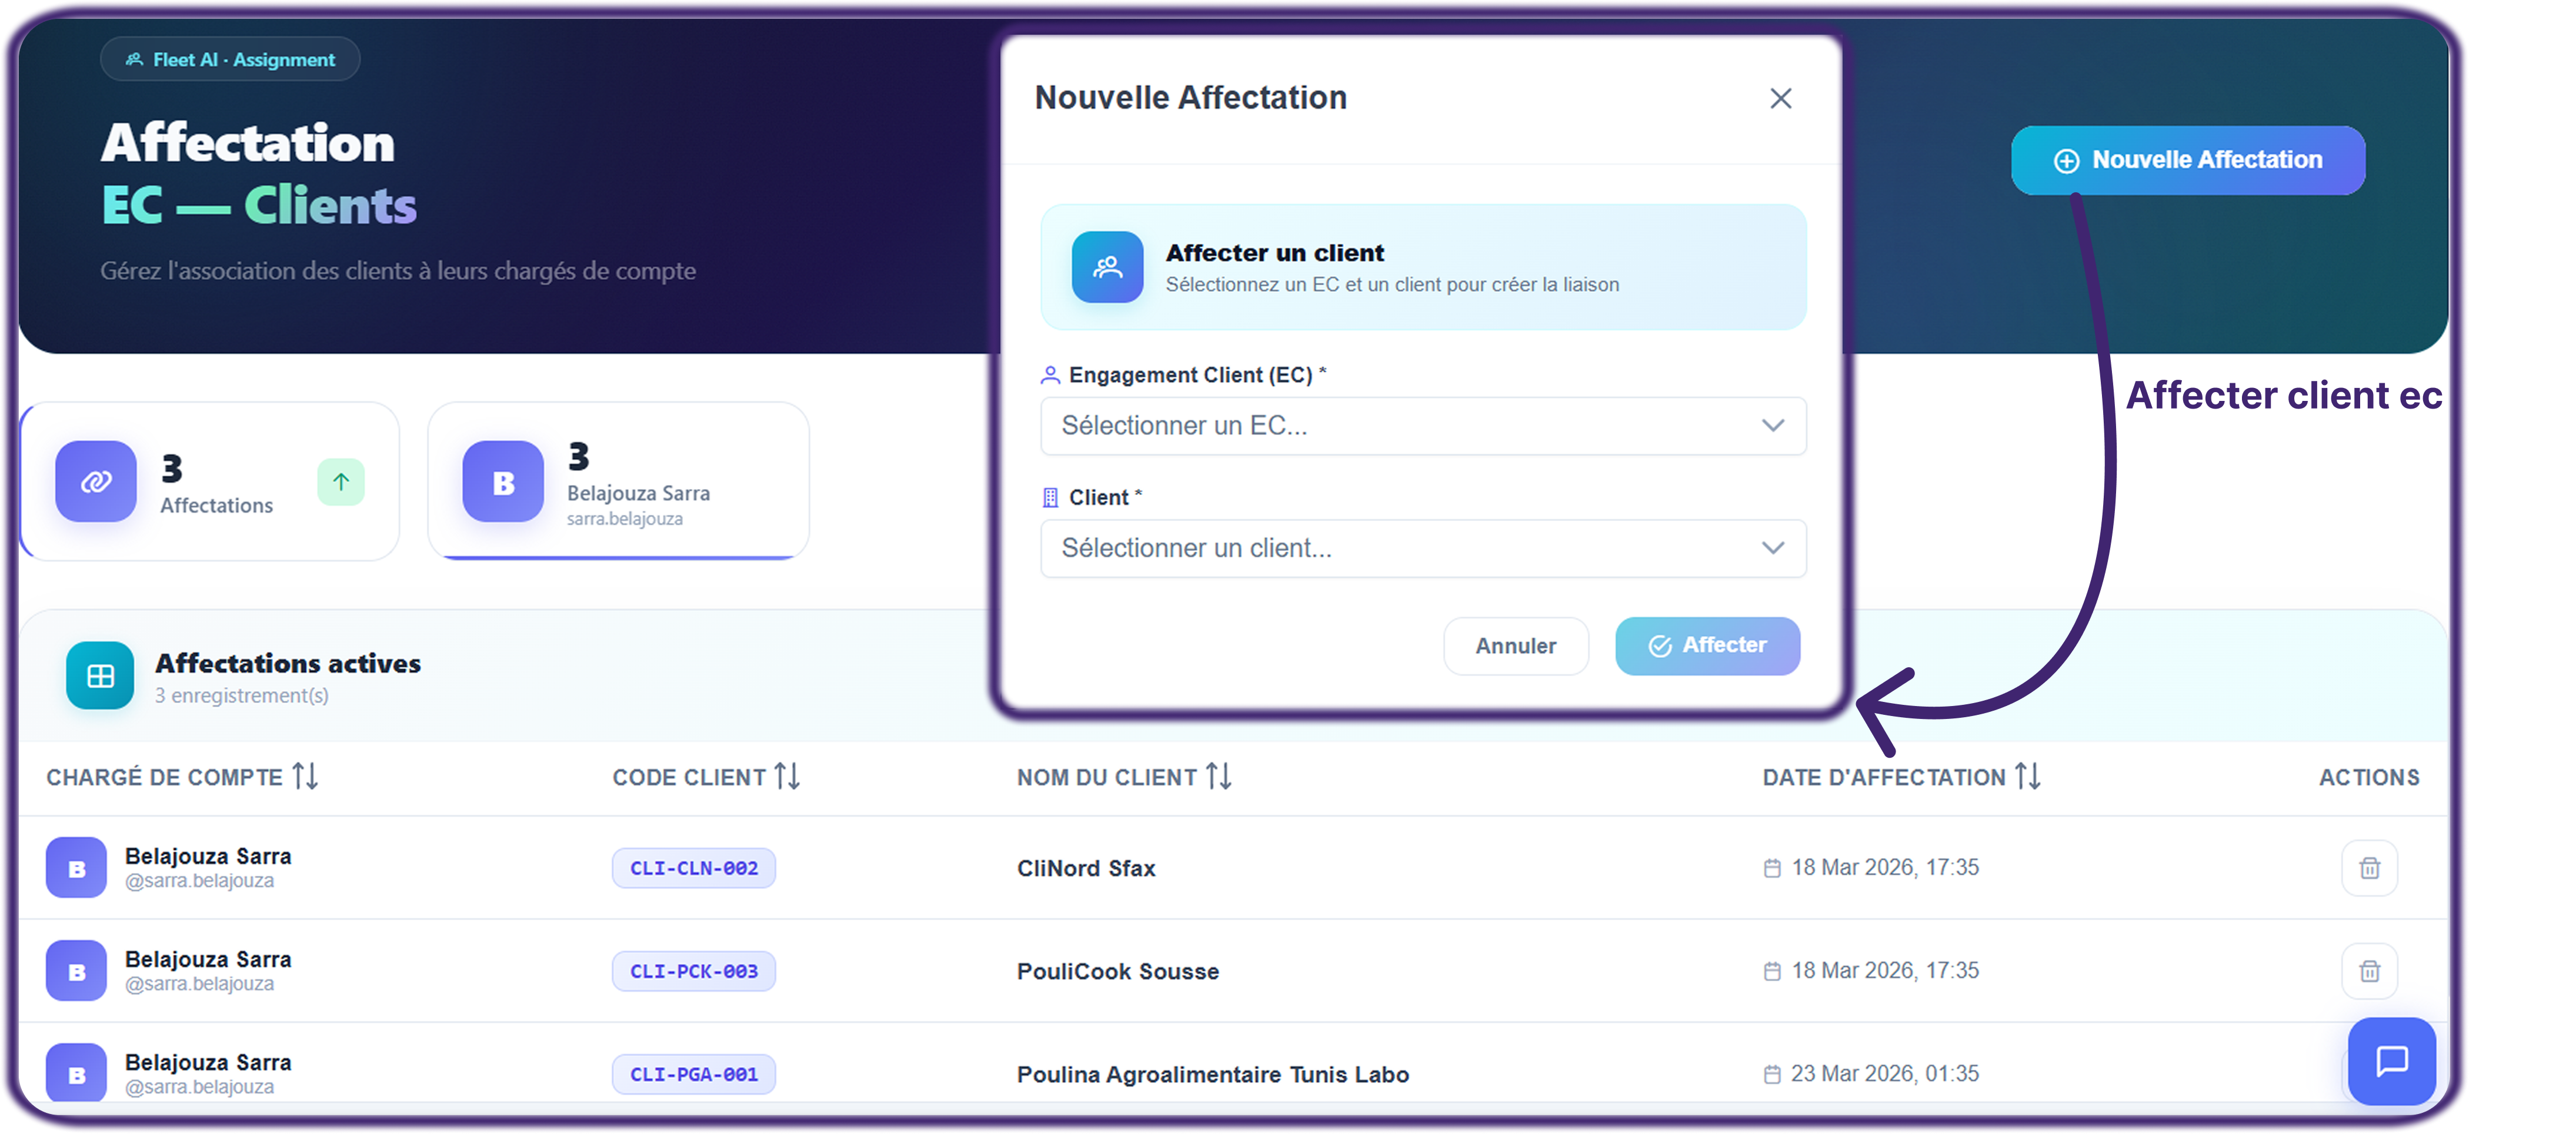
\includegraphics[width=\linewidth, keepaspectratio]{img/capture/web/sp2_ec_assignments_composite}%
}{%
  \fbox{\parbox{0.9\linewidth}{\centering\vspace{1.5cm}\textit{[img/sp2\_ec\_assignments\_composite]}\vspace{1.5cm}}}%
}
\caption{Affectation REC-Client en lot}
\label{fig:sp2-ec-assign}
\end{figure}

\subsection{Application mobile Client (Flutter)}

L'application mobile permet au Client de parcourir le catalogue d'articles, de passer des commandes via un workflow en quatre étapes (catalogue \textrightarrow{} panier \textrightarrow{} adresse \textrightarrow{} type~\&~date de livraison \textrightarrow{} confirmation), et de suivre ses commandes actives avec leur statut en temps réel.

\begin{figure}[H]
\centering
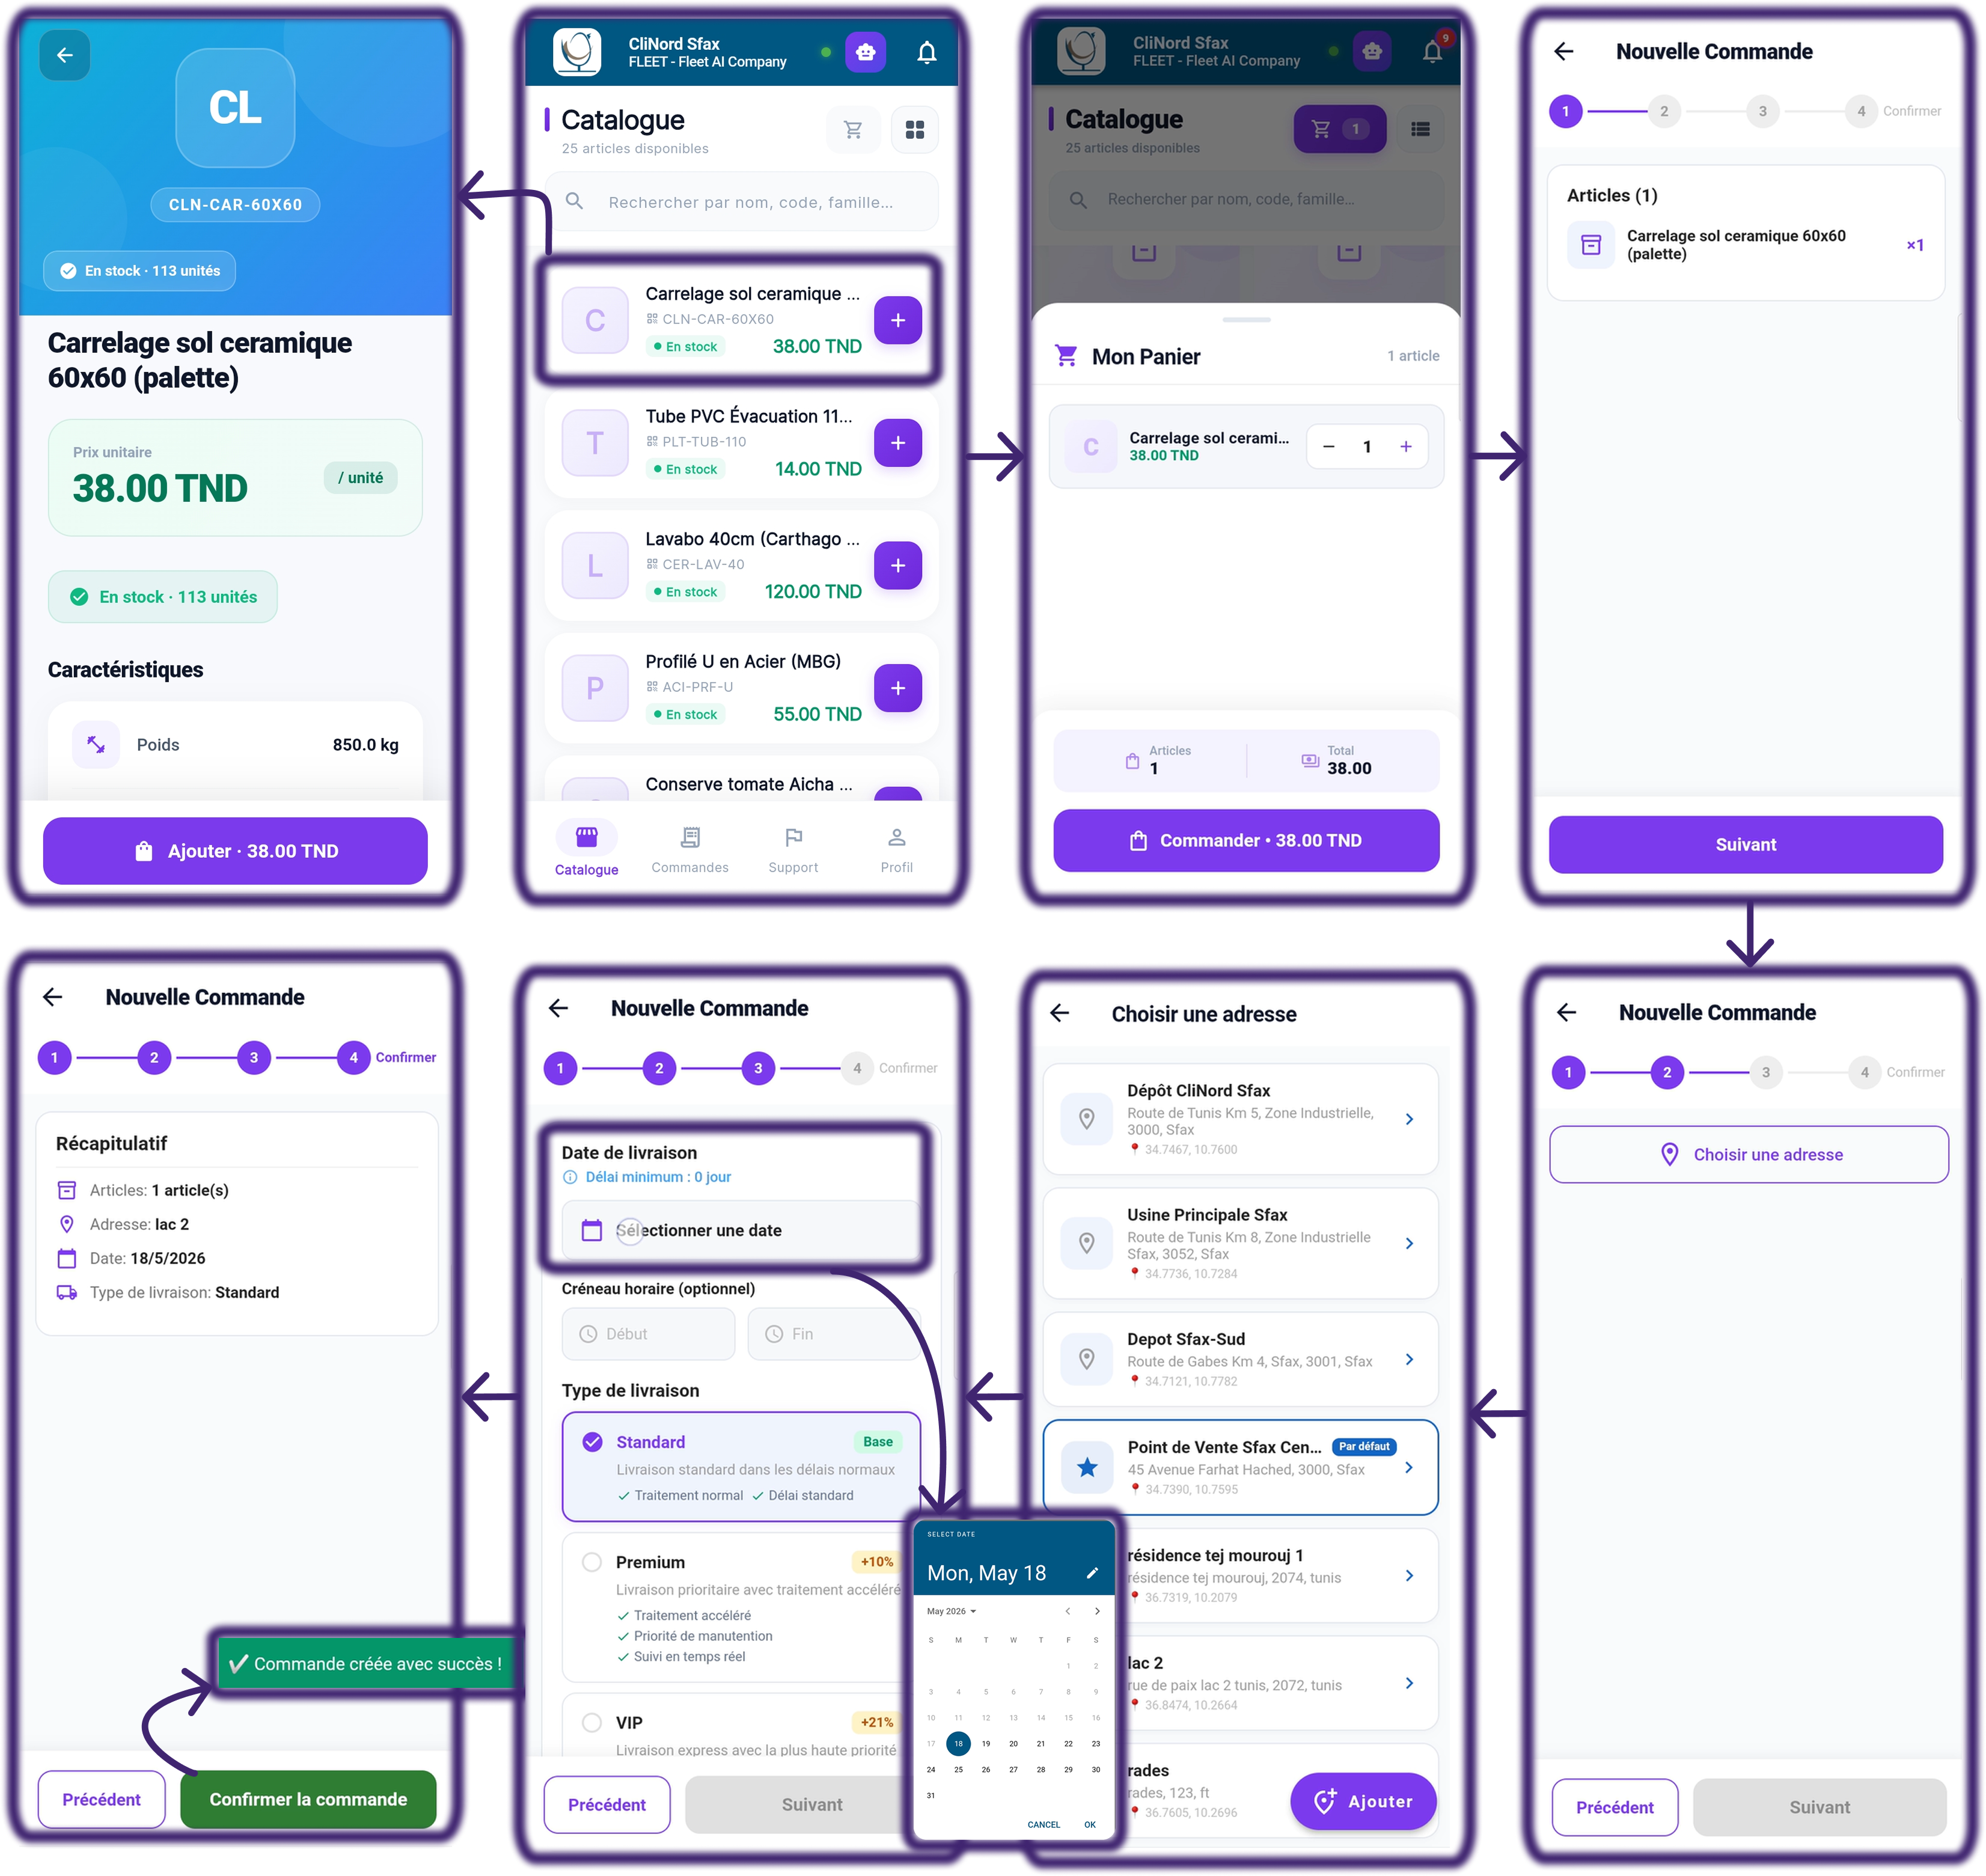
\includegraphics[width=\linewidth, height=0.40\textheight, keepaspectratio]{img/capture/mobile/realisation_commande_client}
\caption{Application mobile Client --- Processus complet de commande : catalogue, sélection d'article, panier, choix de l'adresse de livraison, type de livraison (Standard / Premium / VIP), sélection de créneau horaire et confirmation de la commande}
\label{fig:sp2-mobile-order}
\end{figure}

\begin{figure}[H]
\centering
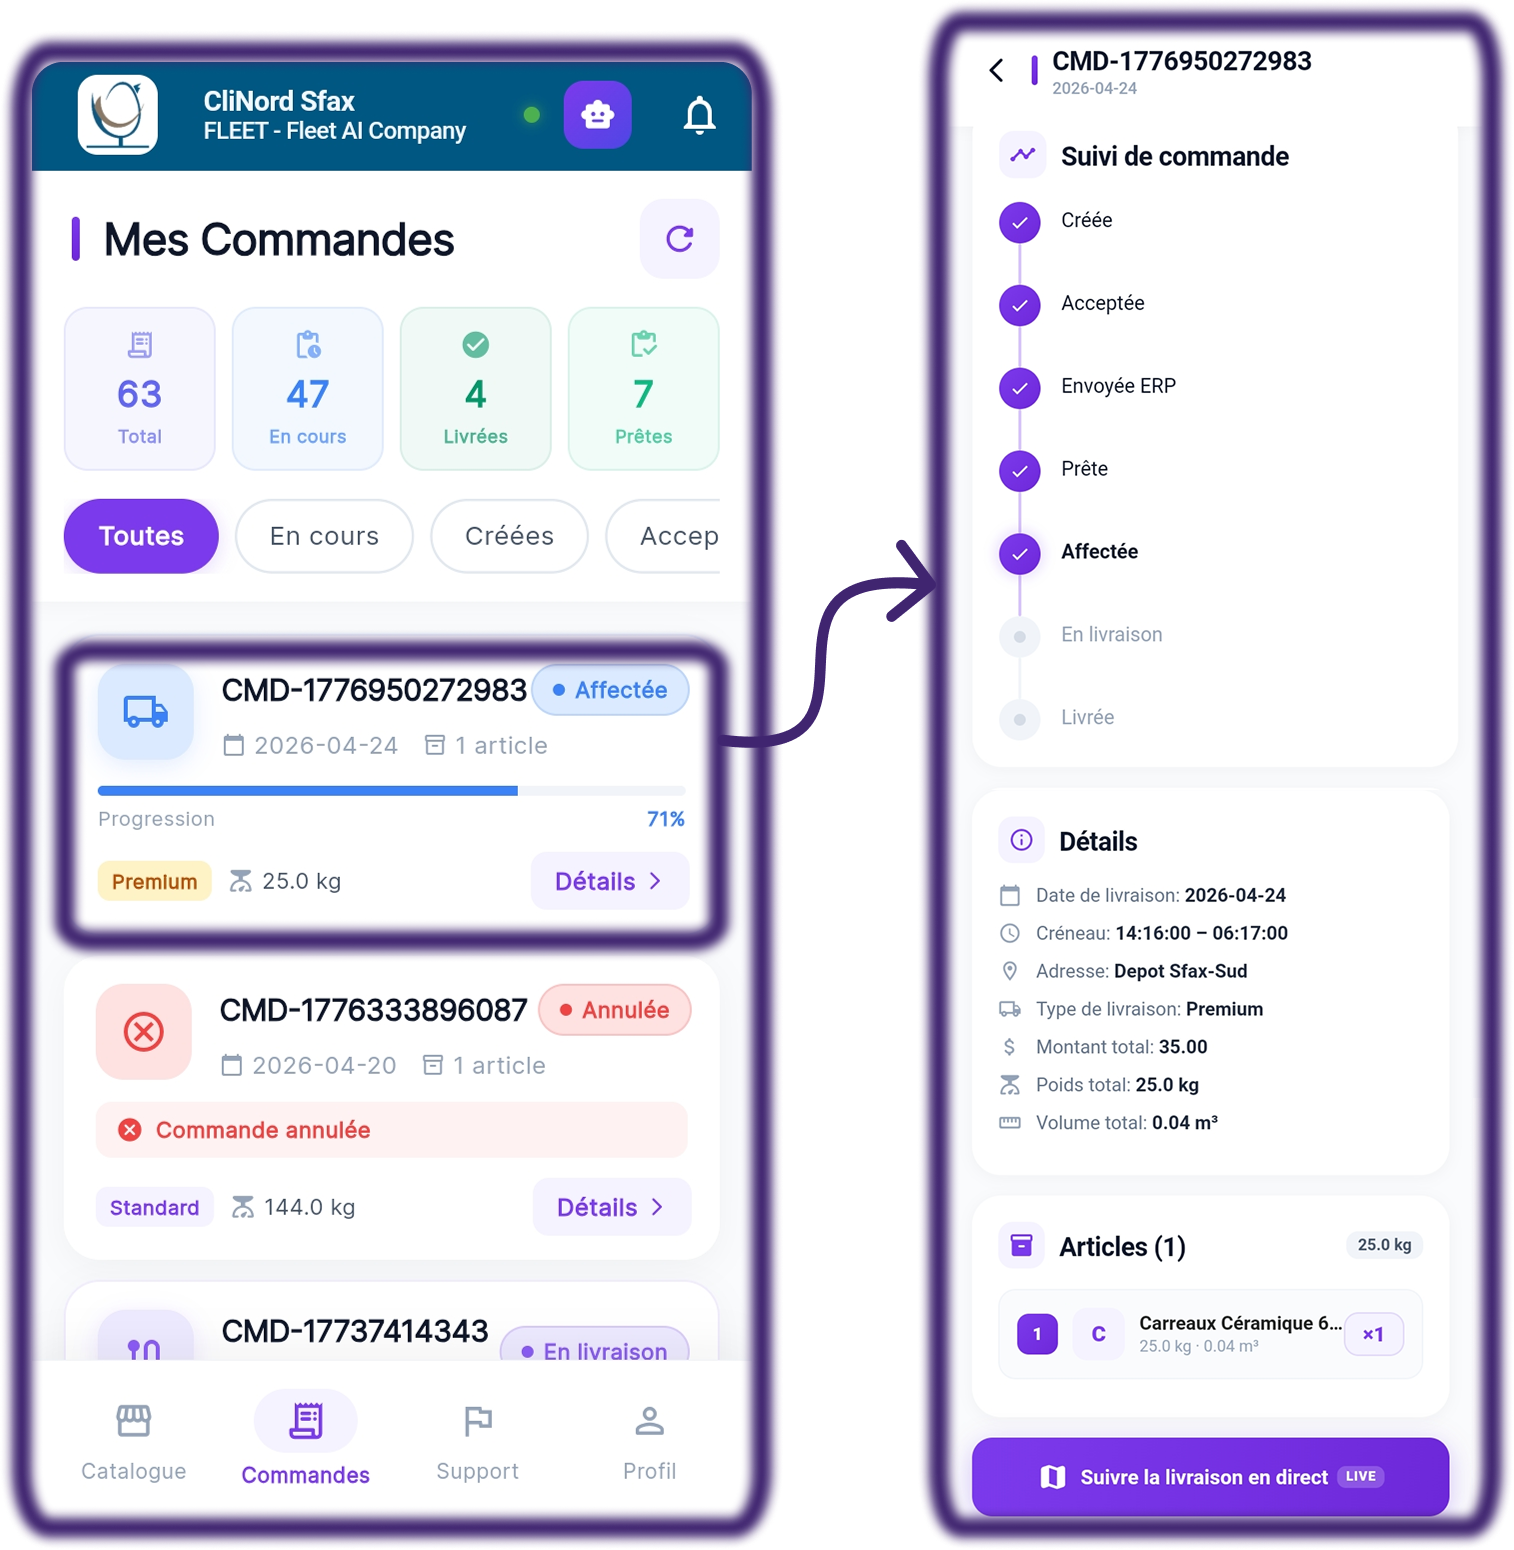
\includegraphics[width=0.55\linewidth, height=0.37\textheight, keepaspectratio]{img/capture/mobile/commande_client}
\caption{Application mobile Client --- Suivi des commandes : liste avec statuts (Affectée, En livraison, Annulée) et détail d'une commande avec progression live}
\label{fig:sp2-mobile-tracking}
\end{figure}

\subsection{Notifications du workflow client}

Le client est notifié automatiquement à chaque changement de statut de ses commandes (commande prête, mise en livraison, livraison échouée) depuis le centre de notifications de l'application mobile. Les notifications sont horodatées et classées par type ; le client peut consulter l'historique complet avec les compteurs (total, non lues, aujourd'hui).

\begin{figure}[H]
\centering
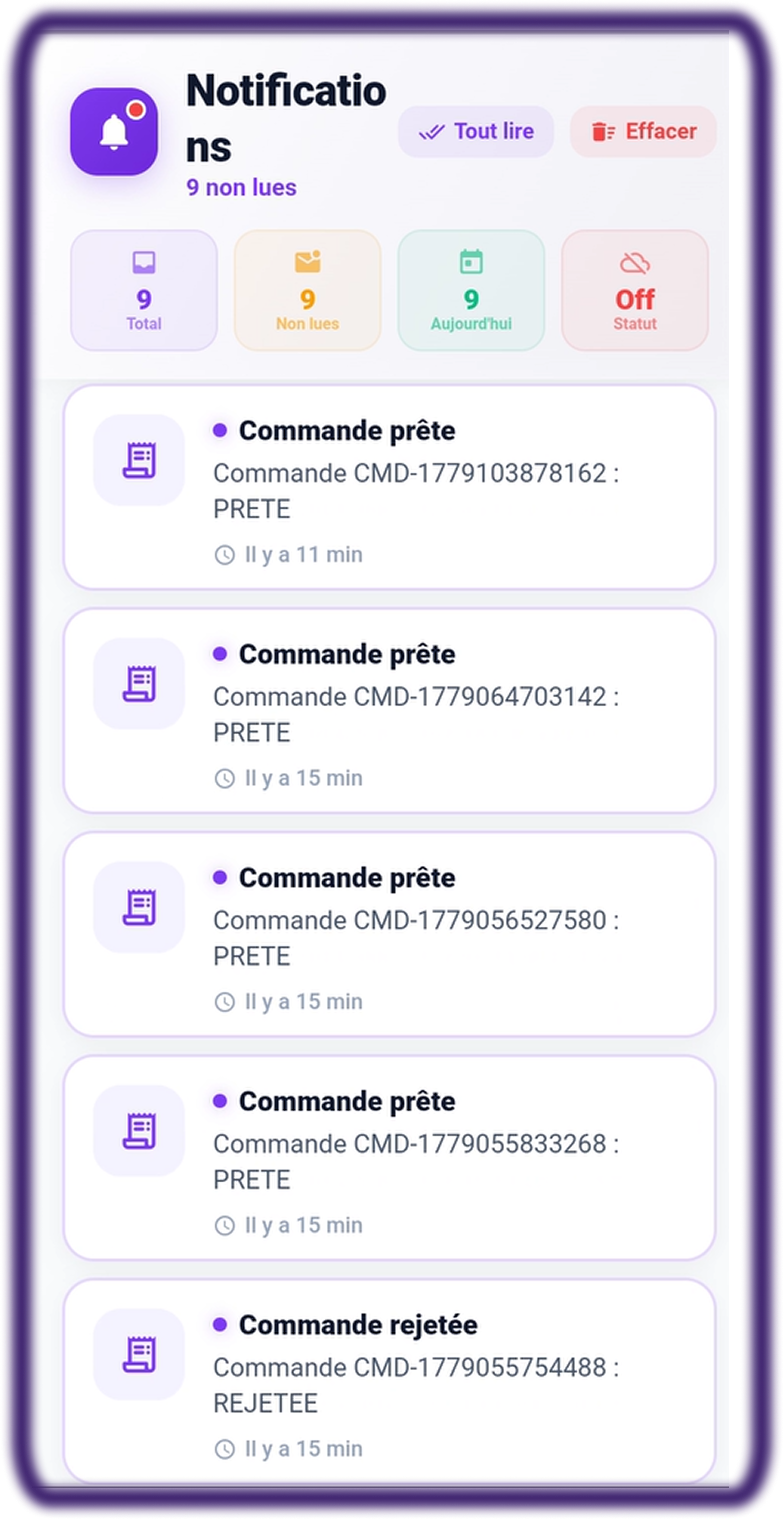
\includegraphics[width=0.40\linewidth, height=0.30\textheight, keepaspectratio]{img/capture/mobile/notification_client}
\caption{Application mobile Client --- Centre de notifications : alertes de statut de commande (prête, rejetée) avec horodatage et compteurs de lecture}
\label{fig:sp2-notification-client}
\end{figure}

\subsection{Profil client et gestion des adresses}

Le Client accède à son profil depuis l'onglet \textit{Profil}. Il y consulte le récapitulatif de ses commandes (total, actives, livrées, annulées) et gère ses adresses de livraison. L'ajout d'une adresse se fait soit manuellement (nom, adresse complète, code postal, ville), soit automatiquement via la géolocalisation GPS («~Utiliser ma position actuelle~»). Une adresse peut être marquée \textit{par défaut} pour être présélectionnée lors des commandes.

\begin{figure}[H]
\centering
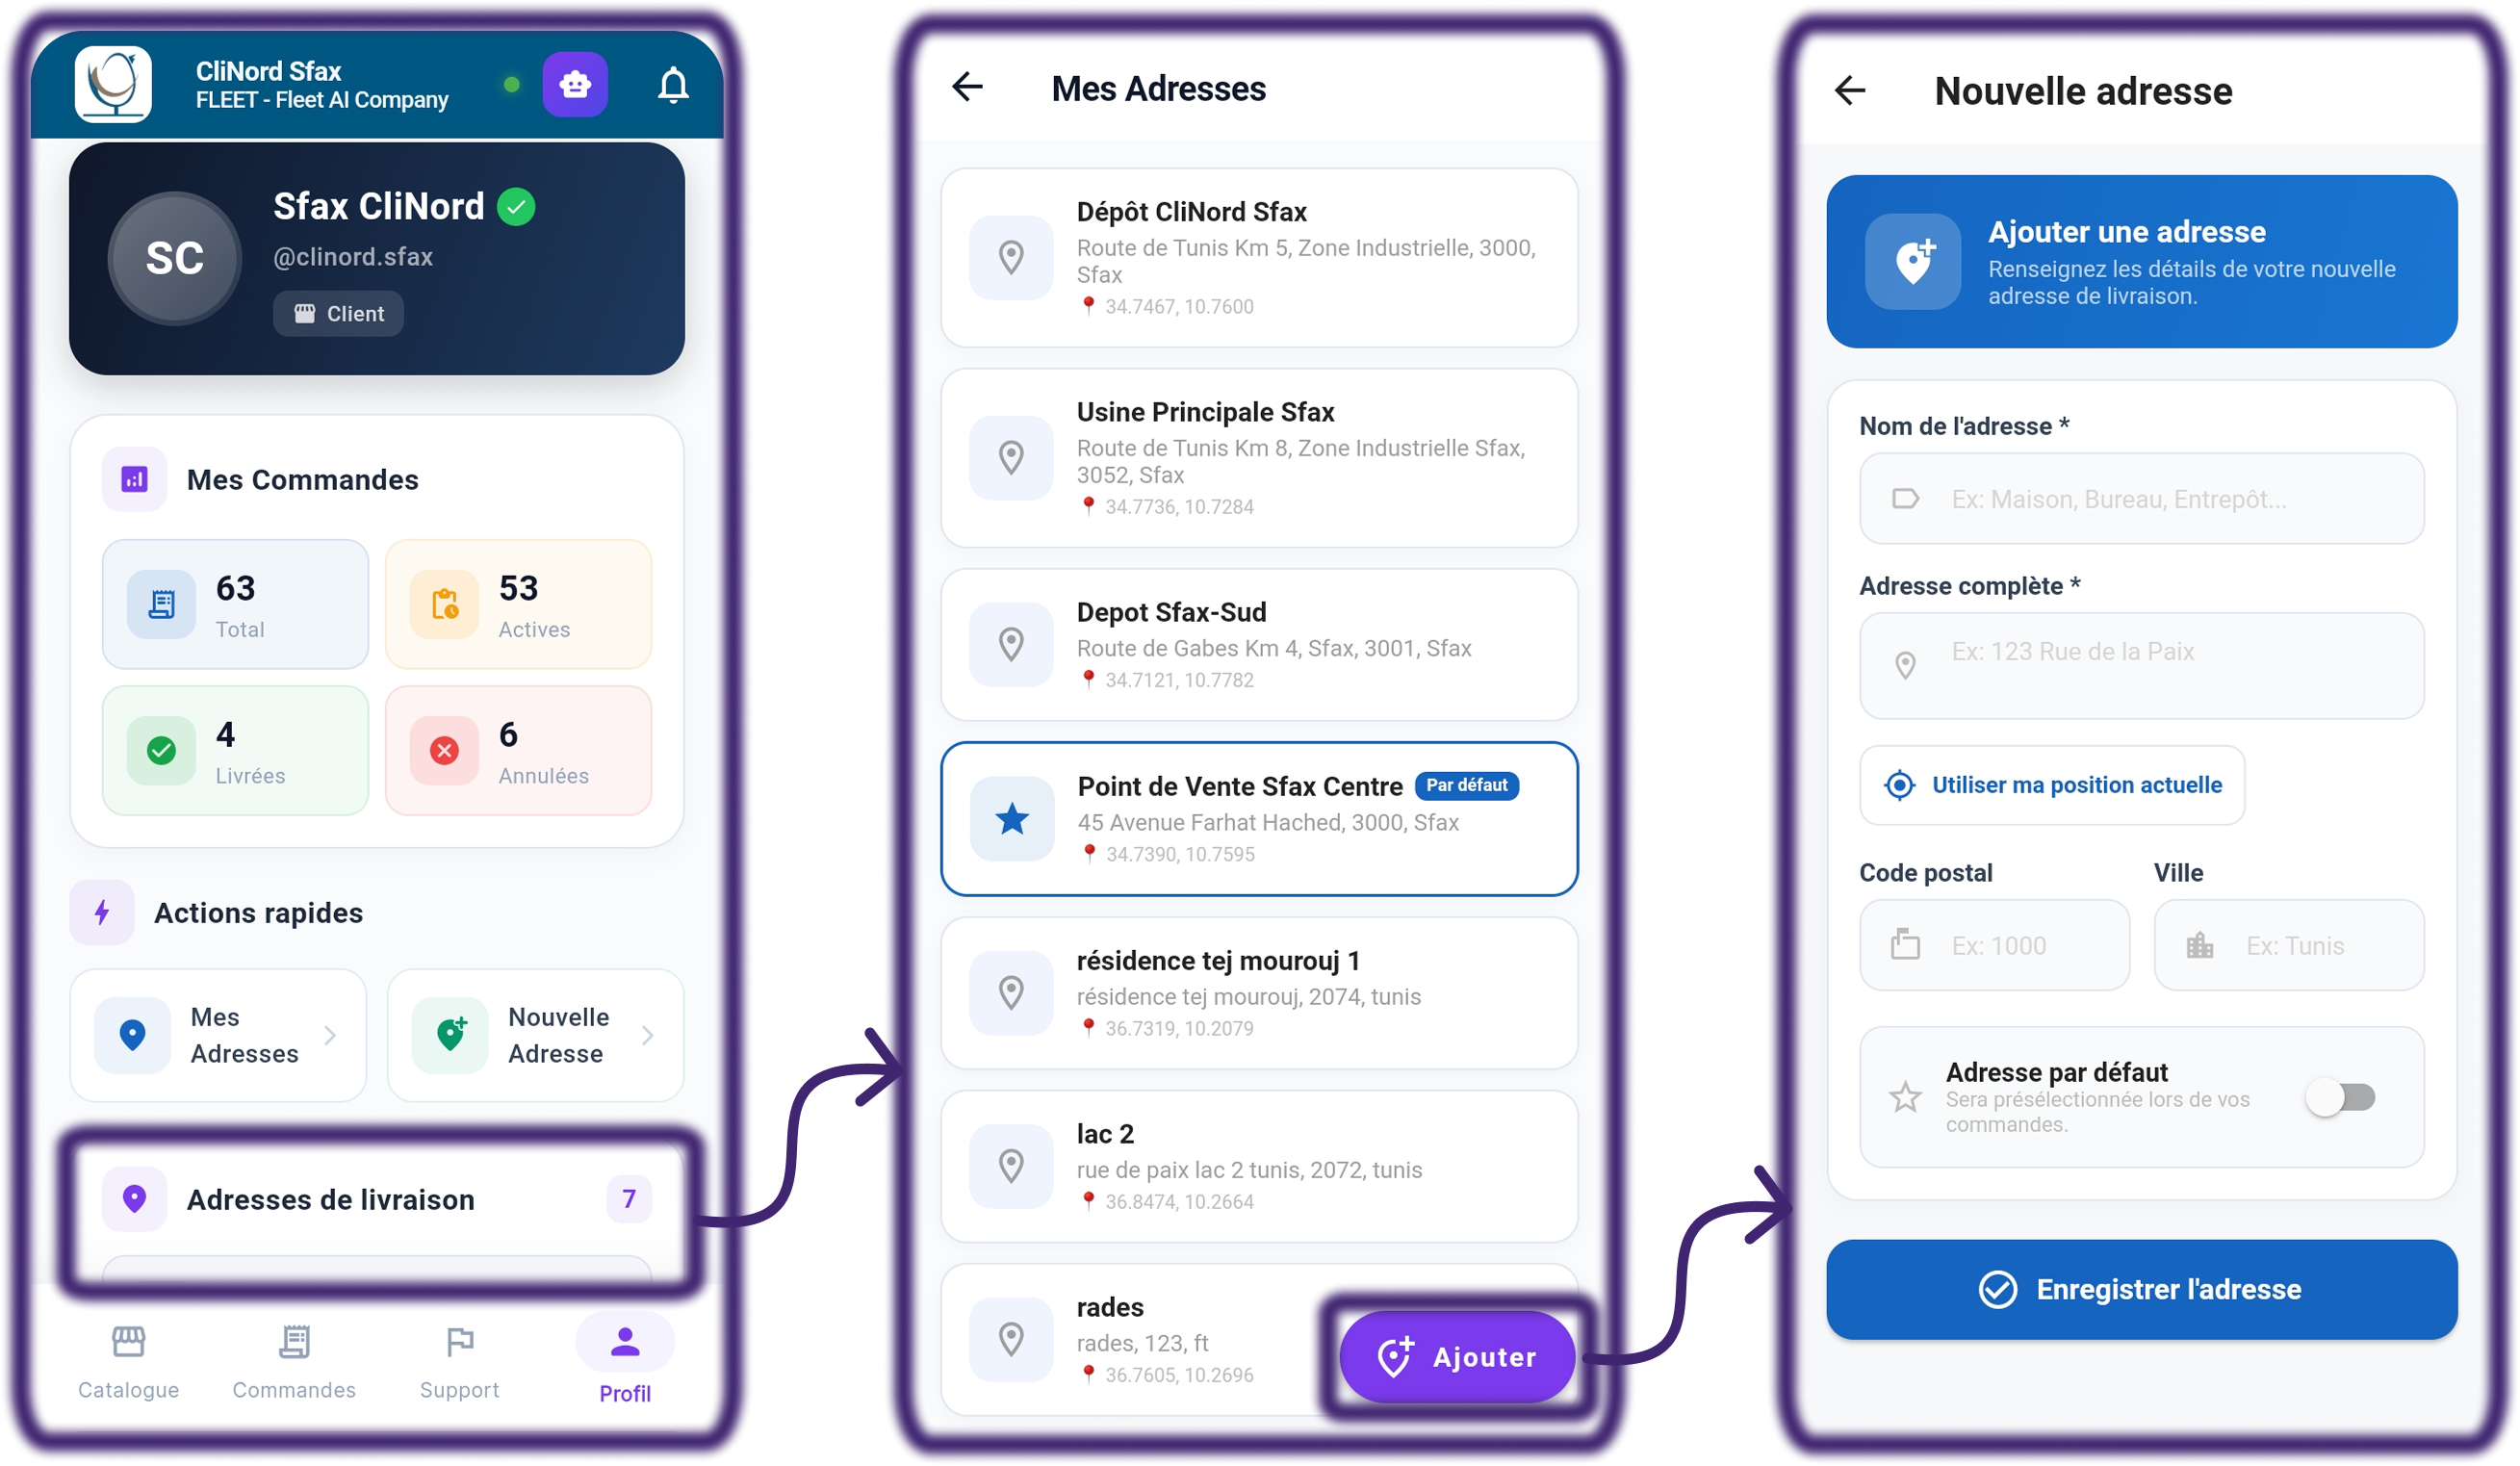
\includegraphics[width=\linewidth, height=0.38\textheight, keepaspectratio]{img/capture/mobile/profile_client}
\caption{Application mobile Client --- Profil et gestion des adresses : récapitulatif commandes, liste des adresses de livraison enregistrées et formulaire d'ajout d'une nouvelle adresse}
\label{fig:sp2-mobile-profile}
\end{figure}

% =============================================================
\section{Tests}
% =============================================================

\begin{figure}[H]
\centering
\IfFileExists{img/capture/web/sp2_test_e2e.png}{%
  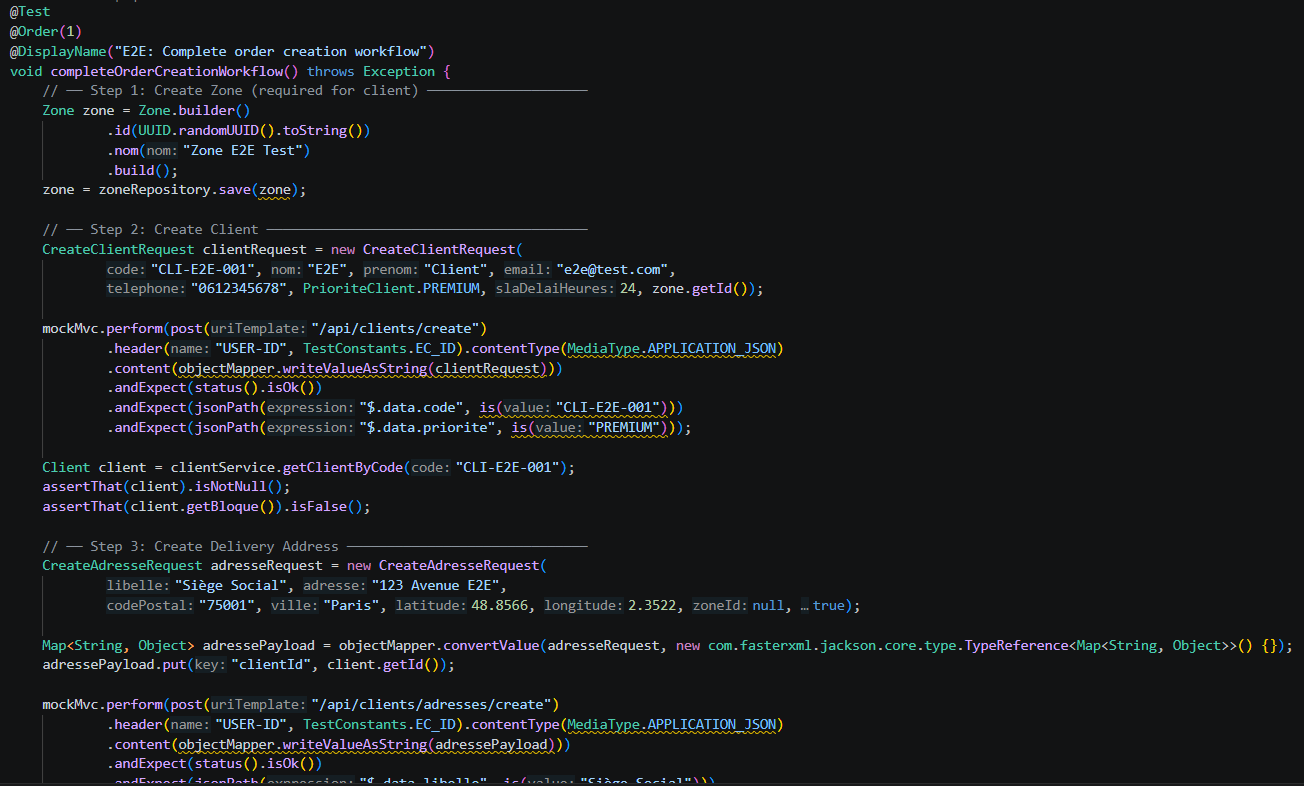
\includegraphics[width=\linewidth, keepaspectratio]{img/capture/web/sp2_test_e2e}%
}{%
  \fbox{\parbox{0.9\linewidth}{\centering\vspace{1.5cm}\textit{[img/capture/web/sp2\_test\_e2e.png]}\vspace{1.5cm}}}%
}
\caption{Exemple d'un test End-to-End (E2E) --- Sprint~2}
\label{fig:sp2-test}
\end{figure}

\begin{figure}[H]
\centering
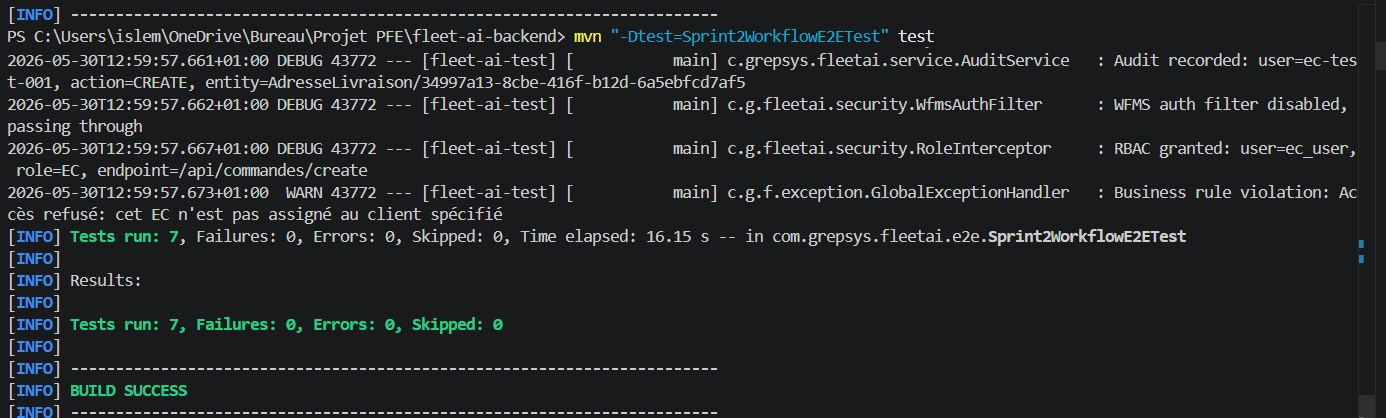
\includegraphics[width=\linewidth, height=0.32\textheight, keepaspectratio]{img/capture/web/sp2_resultat_test_e2e}
\caption{Résultats d'exécution des tests End-to-End --- Sprint~2 (Succès)}
\label{fig:sp2-test-result}
\end{figure}

\section*{Conclusion}
\addcontentsline{toc}{section}{Conclusion}

Le Sprint~2 livre le c{\oe}ur métier de Fleet~AI : gestion des clients, workflow de commandes à dix statuts, stock à deux niveaux et application mobile client. Le Sprint~3 couvre la planification et l'optimisation des tournées.
